%\documentclass[preprint]{aastex}
\documentclass[twolcolumn,apj,iop,numberedappendix]{emulateapj}
%\usepackage{deluxetable}
\usepackage{ctable}
\usepackage{amsmath}
\usepackage{graphicx}
\usepackage{hyperref}
\usepackage{mathrsfs}
%\usepackage[figuresright]{rotating}
%\usepackage{rotating}
%\usepackage{natbib}
%\usepackage{pdflscape}
%\usepackage{lscape}
%\citestyle{aa}

\def\b{\mathbf{b}}
\def\k{\mathbf{k}}
\def\r{\mathbf{r}}
\def\q{\mathbf{q}}
\def\kp{\mathbf{k}^\prime}
\def\kpp{\mathbf{k}^{\prime\prime}}
\def\V{\mathbb{V}}
\def\At{\tilde{A}}
\def\Vt{\tilde{V}}
\def\Tt{\tilde{T}}
\def\tb{\langle T_b\rangle}
\newcommand{\vis}{\mathbf{v}}
\newcommand{\x}{\mathbf{x}}
\newcommand{\xhat}{\hat{\mathbf{x}}}
\newcommand{\A}{\mathbf{A}}
\newcommand{\y}{\mathbf{y}}
\newcommand{\N}{\mathbf{N}}
\newcommand{\Hmat}{\mathbf{H}}
\newcommand{\Nfg}{\mathbf{N}_{\textrm{fg}}}
\newcommand{\Q}{\mathbf{Q}}
\newcommand{\M}{\mathbf{M}}
\newcommand{\W}{\mathbf{W}}
\newcommand{\G}{\mathbf{G}}
\newcommand{\R}{\mathbf{R}}
\newcommand{\F}{\mathbf{F}}
\newcommand{\rhat}{\hat{\mathbf{r}}}
\newcommand{\Nbl}{N_{\textrm{bl}}}

\newcommand{\acl}[1]{{\color{red} \textbf{[ACL:  #1]}}}
\definecolor{applegreen}{rgb}{0.55, 0.71, 0.0}
\newcommand{\mep}[1]{{\color{applegreen} \textbf{[MEP:  #1]}}}

\renewcommand{\topfraction}{0.85}
\renewcommand{\bottomfraction}{0.1}

\begin{document}

%\title{What Power Spectrum Measurements From the Next Generation of 21~cm Experiments Can Teach Us About the Epoch of Reionization}
%\title{Design principles for interferometric measurements of the global $21\,\textrm{cm}$ signal}
\title{Accessing the global $21\,\textrm{cm}$ signal via interferometry}
\title{Measuring the cosmological $21\,\textrm{cm}$ monopole with an interferometer}

\author{Morgan E. Presley\altaffilmark{1},
Adrian Liu\altaffilmark{2,3},
Aaron R. Parsons\altaffilmark{2,4}
}
\altaffiltext{1}{Department of Astrophysical Sciences, Princeton University, Princeton, NJ 08544, USA}
\altaffiltext{2}{Department of Astronomy, UC Berkeley, Berkeley, CA 94720, USA}
\altaffiltext{3}{Berkeley Center for Cosmological Physics, UC Berkeley, Berkeley, CA 94720, USA}
\altaffiltext{4}{Radio Astronomy Laboratory, UC Berkeley, Berkeley, CA 94720, USA}

\begin{abstract}
A measurement of the global 21 cm signal remains a promising but as-of-yet unattained ambition of radio astronomy. Many experiments are proposed or in progress to measure the signal; however, most approaches so far have been single-dipole experiments. In this paper we build off the approach used by LOFAR, which used an interferometric approach based on lunar occultations, and we develop a more general intuition for an optimal design of a radio interferometer array built to measure the global signal. We find that the internal spatial dependence imposed by an antennae beam pattern can induce sensitivity to the global signal. In order to maximize this sensitivity, we find that an array should be constructed as a small, closely-packed, square grid of antennae with full-width-half-max beam sizes of $\sim25^\circ$. We also explore methods of data analysis and propose a two-step process that estimates the monopole at each frequency channel and then does a final foreground subtraction on the entire estimated spectrum. Within this method we propose estimating the monopole using a method that minimizes the variance and preserves the amplitude of a pure monopole sky. When we put our array design and data analysis method into numerical simulation, we find that an interferometric measurement of the global signal is comparable to a single-dipole experiment. \mep{Perhaps add a few numbers when nersc finishes running.}

\end{abstract}


\keywords{reionization, dark ages, first stars --- techniques: interferometric}

\section{Introduction}
\acl{DID WE REMEMBER TO DIVIDE THE $a_{00}$ values by $\sqrt{4\pi}$?}
\acl{Check contour levels}

While recent years have marked tremendous progress in astronomical measurements at increasingly high redshifts, still missing are direct observations of our Universe when the first generation of luminous objects were being formed. Such observations would provide constraints on crucial periods in our cosmic timeline, including the epoch of reionization, when the intergalactic medium (IGM) experienced a large-scale phase transition, changing from neutral to almost fully ionized. Optical and infrared observations at $z \lesssim 7$ have provided some constraints on the end stages of reionization, but have difficulties probing its early to intermediate stages. Moreover, modeling uncertainties often make observations difficult to interpret. Cosmic microwave background (CMB) experiments are sensitive to secondary anisotropies sourced by reionization, but the resulting constraints are based on measurements integrated along one's line-of-sight and are at best rather coarse probes of the relevant astrophysics. These existing probes have even more difficulty pushing beyond reionization to the earlier epoch known as the dark ages, during which time the first stars were formed.

One promising way to directly observe both reionization and the dark ages would be to make use of the $21\,\textrm{cm}$ hyperfine transition of hydrogen. By statistically measuring the brightness temperature of the $21\,\textrm{cm}$ line, one probes both the distribution of large scale structure (using atomic hydrogen as a tracer) and the ionization state of the IGM. Given the abundance of neutral hydrogen at a broad range of redshifts through the end of reionization, the $21\,\textrm{cm}$ line is an ideal way to place direct constraints on the first luminous objects and how they affected their surroundings. Moreover, the spectral nature of $21\,\textrm{cm}$ measurements not only allows a three-dimensional reconstruction of the brightness temperature distribution, but also provides information on its evolution.


\begin{figure*}[!]
	\centering
	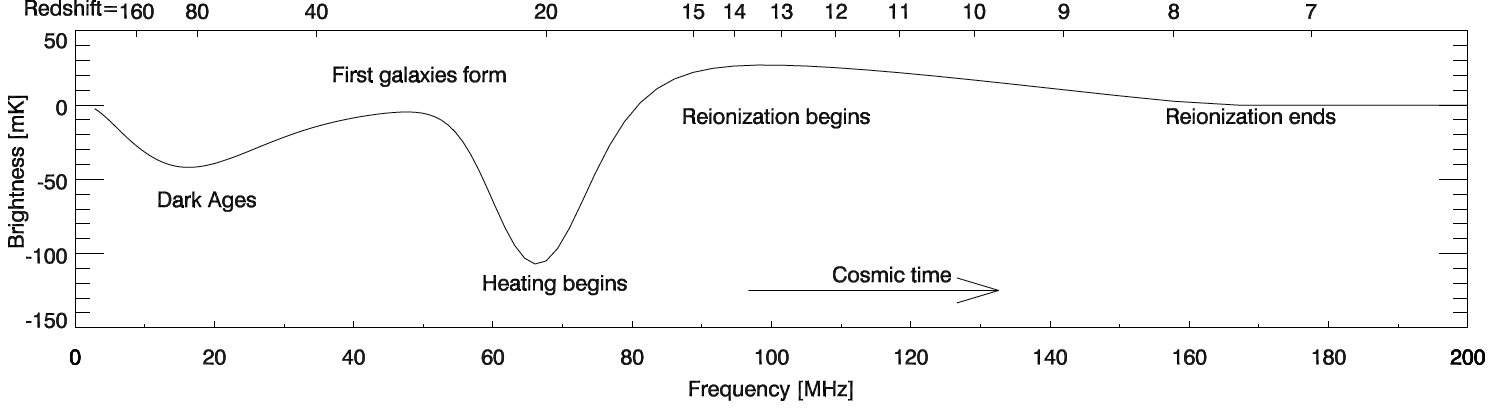
\includegraphics[width=1.00\textwidth]{figures/fidModel.png}
	\caption{A fiducial model of the global 21 cm signal, as modeled in \citet{PritchardLoeb2010}. Although this model should capture the essential features of the signal, the precise details have yet to be confirmed and depend on the nature of the first stars and galaxies.}
	\label{fig:21cmSignal}
\end{figure*}

Just as with the CMB, the $21\,\textrm{cm}$ line can be characterized by a mean brightness temperature (obtained by averaging the cosmological signal in angle over the entire sky) and anisotropic fluctuations about this mean. However, unlike the CMB, the mean $21\,\textrm{cm}$ brightness temperature does not follow a simple blackbody spectrum. Instead, this ``global $21\,\textrm{cm}$ signal" is richly dependent on the astrophysics of the dark ages and reionization. Figure \ref{fig:21cmSignal} shows a schematic of a fiducial model of the global 21 cm signal, highlighting the important epochs and corresponding features in the signal. The first epoch, the cosmic ``dark ages,'' arises with the thermal decoupling of the 21 cm spin states from the cosmic microwave background (CMB) and is marked by a shallow absorption feature. As the gas density continues to fall with the universe's expansion, collisions are no longer able to couple the spin states to the gas, and the signal falls back into coupling with the CMB. The next epoch is marked by the formation of the first stars and galaxies, whose Ly$\alpha$ photons strongly couple the spin states to the gas temperature. This first results in a deep absorption feature, as the gas temperature is far below that of the CMB. However, heating from X-ray emission pushes the gas above the CMB temperature, resulting in a 21 cm emission signal. This leads to the final epoch, the ``epoch of reionization,'' where UV photons ionize the gas, gradually erasing the 21 cm signal. \mep{Do I need to cite \citet{Pritchard_Loeb_21cm_Review} since I used them for reference when writing this?} 

A measurement of the 21 cm global signal would also have the potential to rule out other, non-fiducial models such as those involving dark matter annihilations or stellar black holes. Dark matter annihilation scenarios provide heating beyond that from X-ray emission, and hence dampen the absorption and emission signals at the end of the dark ages and during the epoch of reionization. \citep{Valdes2013_DM} Similarly, ionizing photons from accreting stellar black holes might also add significant heating. Work by \citet{Mirabel_stellar_bh} suggests that including the effects of black holes would cause the 21 cm emission signal to occur earlier than otherwise expected and would also shorten the width of the absorption feature. A global 21 cm measurement would be able to detect evidence for or against such models. 

\begin{itemize}
\item Challenge of foregrounds.  \acl{We should probably also comment on the ionosphere at some point}.
\item Survey of current instruments and efforts. (EDGES, DARE, SCI-HI, LOFAR, LEDA, LWA) \acl{Gotta also survey some of the other experiments that one doesn't hear about so much.  Gianni's paper has a good list.  Also be sure to add more references like Jack Burns' ScienceDirect article.}
\end{itemize}
There are currently a large number of experiments seeking to make a first detection and characterization of the global $21\,\textrm{cm}$ signal.  The Experiment to Detect the Global EoR Signal (EDGES) uses an extremely well-calibrated single dipole \citep{rogersCalib} to integrate over large parts of the sky, producing a global spectrum from $100$ to $200\,\textrm{MHz}$.  Modeling foreground spectra as a sum of low-order polynomials, EDGES has placed a lower limit of $\Delta z > 0.06$ on the duration of reionization \citep{bowmanRogersMeasurement}.  Similar in concept but operating at a lower frequency range of $55$ to $99\,\textrm{MHz}$ is the Sonda Cosmol\'{o}gica de las Islas para la Detecci\'{o}n de Hidr\'{o}geno Neutro (SCI-HI) experiment.  This frequency range corresponds to the redshift range $13.3 < z < 24.9$, providing access to the prominent dip in the signal prior to reionization.  Using a similar polynomial foreground subtraction technique to EDGES, SCI-HI is able to achieve a foreground residual level of $\sim 10\,\textrm{K}$ at $\sim 70 \,\textrm{MHz}$ \citep{voytekSCIHI}.

To escape radio frequency interference (RFI), both EDGES and SCI-HI are deployed in rather remote locations: EDGES observes from the Murchison Radio-astronomy Observatory in Western Australia, while SCI-HI has been deployed at Isla Guadalupe in Mexico, with plans to observe at Isla Socorro and/or Isla Clari\'{o}n in the future.  To achieve even better RFI isolation (as well as to escape ionospheric distortions), the Dark Ages Radio Explorer (DARE) satellite has been proposed \citep{DAREMCMC}.  DARE consists of a short dipole antenna in lunar orbit, which allows the Moon to be used an RFI shield.  DARE probes a frequency range of $40$ to $120\,\textrm{MHz}$, again providing direct access to the pre-reionization epoch.

Moving beyond single dipole experiments, the Large-aperture Experiment to detect the Dark Ages (LEDA) makes use of an interferometric array of antennas to simultaneously model the sky and calibration parameters \citep{BernardiLEDA}.  Fundamentally, however, its measurement of the global signal is still expected to come from total power measurements (i.e., auto-correlations) from single dipoles treated independently.  This differs from the approach taken by \citet{VedanthamLOFAR2}, where the LOw Frequency ARray (LOFAR) was operated as a true interferometer not just for calibration purposes, but also for the cosmological measurement itself.  At a basic level, one might imagine that interferometers are sensitive only to spatially fluctuating signals on the sky (if one follows the standard procedure of avoiding noise bias by discarding auto-correlations in the data), and are therefore insensitive to the global signal.  However, an externally imposed spatial dependence can introduce sufficient spatial structure for a global signal to be measurable by an interferometer.  \citet{VedanthamLOFAR2} took advantage of this fact by observing fields containing the Moon, effectively using lunar occultations to introduce the necessary spatial dependence for an interferometric measurement of the global signal.  So far, this approach has yielded a reasonably high signal-to-noise characterization of the foreground contaminants between $\nu =35$ and $80\,\textrm{MHz}$.

\begin{itemize}
\item Why an interferometer might be helpful plus why we're not crazy (Ekers + Rots Theorem?).  Angular info helps with foreground suppression.
\end{itemize}
\acl{Somewhere, need to address the point that time integration can allow extra information to be gleaned.}

In this paper, we build on \citet{VedanthamLOFAR2}, generalizing their work to consider a general theory of interferometric measurements of the global $21\,\textrm{cm}$ signal.  We provide a mathematically rigorous framework for extracting the global signal from an interferometer.  Given that interferometers naturally sample spatial information, a global signal measurement that is made by an interferometer is well-poised to use angular information to separate foregrounds from the (monopole) cosmological signal.  As pointed out in \citep{L13} and \citep{Liu_Switzer_2014}, the angular dependence of foregrounds can be leveraged to enable better foreground subtraction.  In this present paper we use our mathematical formalism to show how such a scheme may be implemented in the specific context of an interferometric measurement.  Although we find that some amount of spectral foreground subtraction is still necessary, our Monte Carlo simulations show that spatial information can reduce the burden of the spectral subtraction, reducing the risk of cosmological signal loss.  \acl{Should probably have brought up cosmological signal loss and angular subtraction earlier}  Fisher matrix projections confirm the stringent constraints on the dark ages and reionization that can be obtained with our approach.  \acl{Probably want a statement stronger than this.}

\begin{itemize}
\item Preview results (exquisite extraction; great foreground mitigation; high significance detection).
\end{itemize}

The rest of this paper is organized as follows.  In Section \ref{sec:BackOfEnvelopeArrayDesign} we provide some qualitative intuition for using interferometry to measure monopole signals.  This is made more mathematically rigorous in Section \ref{sec:MathForm}, where we establish a matrix-based framework for signal extraction.  Section \ref{sec:Foregrounds} introduces foregrounds and our strategy for their mitigation.  Its effectiveness is demonstrated using Monte Carlo simulations in Section \ref{sec:MonteCarlos}.  The Monte Carlo results are then propagated through to theory parameters in Section \ref{sec:Fisher} using a Fisher matrix formalism.  We summarize our conclusions in Section \ref{sec:Conc}.
\acl{Gotta talk about systematics like RFI, cross-talk, noise bias, etc.}
\acl{Insert guide for readers who don't like math.}

%\section{Why we're really not crazy}
%\label{sec:QualitativePic}
%\begin{itemize}
%\item Cartoon / qualitative picture? \mep{Remind me -- What was this pic supposed to show?}
%\item Simple eqn. showing that there is non-zero response?
%\item Intuitive, qualitative description of what sort of arrays are good.  (Preview for later sections).
%\item Discussion of noise bias and other problems with single dipole experiments?
%\end{itemize}

\acl{A quick reminder of knobs that we can turn: array spacing, beam size, beam size frequency dependence, spectral indices, spectral index spread, higher curvature components etc.}

\acl{Figure out what spread is realistic for low frequency measurements}

\section{Back-of-the-envelope array design}
\label{sec:BackOfEnvelopeArrayDesign}

In this section, we use simplified toy models to build intuition for the types of interferometer arrays that are best suited for probing the global signal.  The goal here is to provide a rough sense for what might be a sensible design that we will analyze in a more numerically detailed fashion in the rest of the paper.

\subsection{A qualitative picture of a global signal interferometer}

Consider first a purely qualitative picture of a two-element interferometer. An interferometer measures the sky convolved with the antennae's beam pattern and with the spherical harmonic corresponding to the interferometer's baseline. Without the beam pattern it would be impossible to measure a monopole signal since a constant convolved with a spherical harmonic returns zero. However, as shown schematically in Figure \ref{fig:beam_pattern_cartoon}, when the beam pattern is added into the convolution, its enveloping effect will prevent the convolution from integrating to zero, making an interferometer sensitive to the monopole signal. 

An equivalent way to look at the problem is to move into spherical-harmonic space and examine the $uv$ plane, shown in Figure \ref{fig:uv_cartoon}. An interferometer with baseline length $\b$ will measure the sky at the point $\mathbf{u} = \frac{\nu\b}{c}$ in the $uv$ plane. To measure the monopole, one must recover information from the origin, which corresponds to a zero-length baseline. This is possible because the convolution with the beam pattern smears out the point of measurement (i.e. the measurement incorporates information from other nearby baselines), with narrower beams corresponding to larger smears. As shown by the green circle in Figure \ref{fig:uv_cartoon}, if the baseline is short enough and the beam is narrow enough, then the measured signal will include information from the global signal. 

In the rest of Section \ref{sec:BackOfEnvelopeArrayDesign} we will make this qualitative picture more mathematically precise and develop an array design that will maximize sensitivity to the global signal and minimize contamination from foregrounds and other spherical harmonic modes. 
 
\begin{figure}[h]
	\centering
	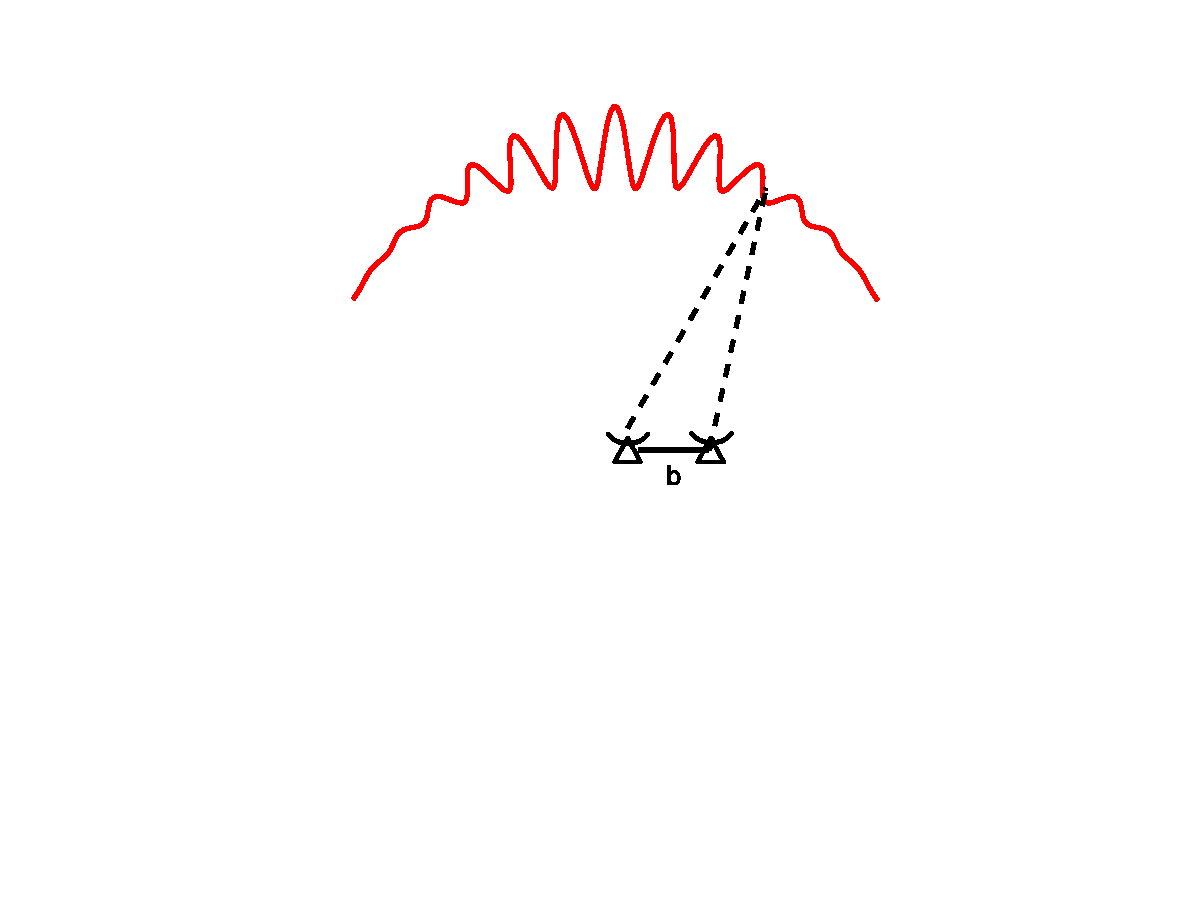
\includegraphics[width=0.50\textwidth]{figures/beam_pattern_cartoon.pdf}
	\caption{A schematic illustration of a two-element interferometer. The two antennae, separated by a baseline length $\b$, measure a spherical harmonic on the sky, shown as a cosine function on an arc. This function would integrate to zero over the entire sky. However, the antennae also produce a beam pattern which is strongest at the zenith and fades to the horizon. Due to this envelope, a monopole signal convolved with the beam pattern and spherical harmonic will not return zero when integrated over the entire sky. Therefore, an interferometer will in fact be sensitive to a monopole signal.}
	\label{fig:beam_pattern_cartoon}
\end{figure}

\begin{figure}[h]
	\centering
	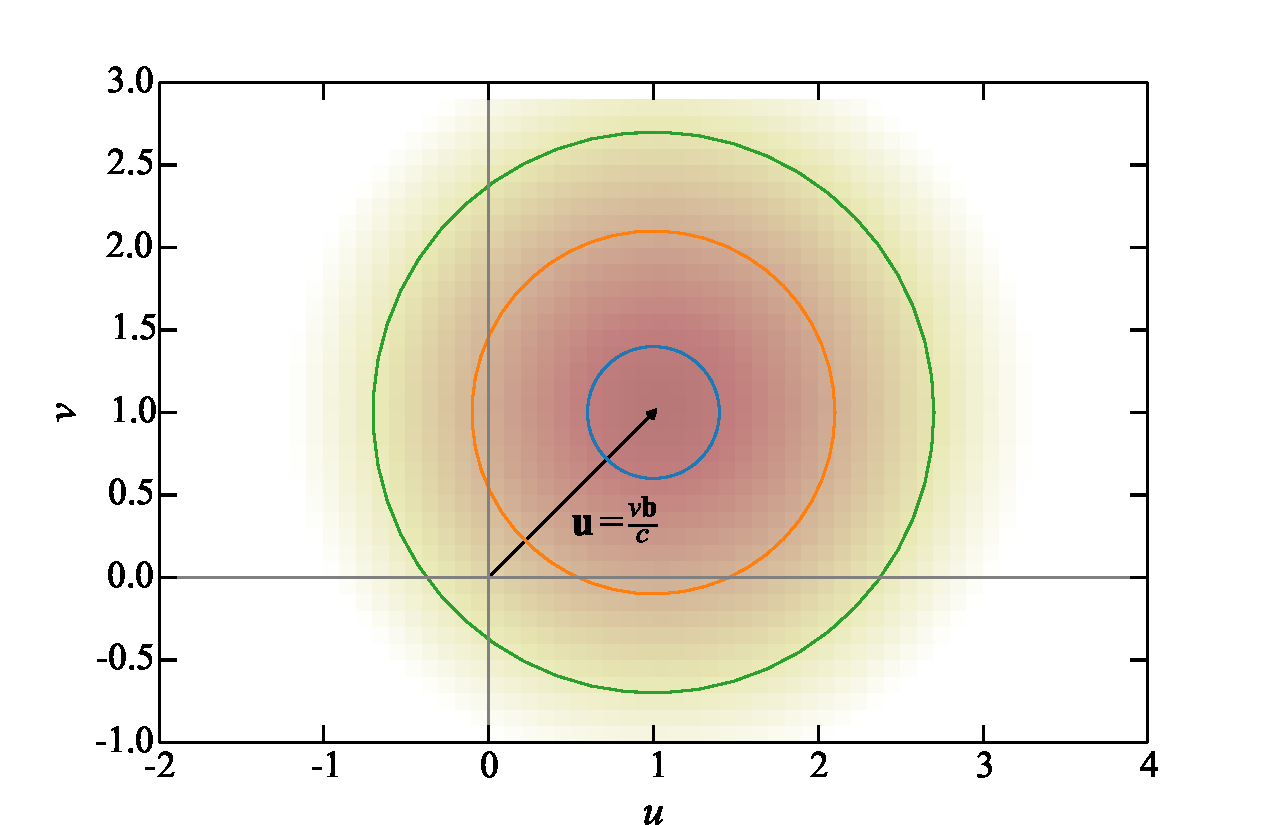
\includegraphics[width=0.50\textwidth]{figures/uv_cartoon.pdf}
	\caption{A schematic illustration of the $uv$ plane for an interferometer. Since the uv plane represents baselines in Fourier space, an interferometer with baseline $\b$ makes a measurement at the point $\mathbf{u} = \frac{\nu\b}{c}$. Measuring the monopole signal would require making a measurement at the origin of the uv plane, which is probed by a baseline of zero length. This seems impossible until one recalls that a real interferometer does not measure an exact point: the antenna's beam pattern smears the measurement in the uv plane, so that the measurement contains information from nearby baselines. Since a narrower beam corresponds to a larger smear, two narrow-beam antennae placed close together would make a measurement that incorporates information from the monopole, as shown by the green circle in the figure.}
	\label{fig:uv_cartoon}
\end{figure}


\subsection{Sparse or packed arrays?}

Suppose we consider an array consisting of just a single baseline, and ask what baseline length $b$ optimizes measurements of the global signal.  Intuitively, a short $b$ increases sensitivity to the signal, since (for a given $uv$ plane primary beam kernel) short baselines have the greatest overlap with the $\mathbf{u}=0$ mode, which is precisely what we are seeking to measure.  On the other hand, foregrounds contamination is worst for short baselines, since they are mostly sensitive to the smoothest spatial modes of the sky, where foregrounds dominate.  There must therefore exist an intermediate baseline length that best balances these two competing demands, which we will now compute.

In the flat-sky approximation, the visibility response $V(\mathbf{b})$ of a baseline $\mathbf{b}$ to the sky temperature $T(\boldsymbol \theta)$ is given by
\begin{equation}
\label{eq:Vb}
V(\mathbf{b}) = \int  T(\boldsymbol \theta) A(\boldsymbol \theta) \exp \left( -i 2 \pi \frac{\nu}{c} \mathbf{b} \cdot \boldsymbol \theta \right) d^2 \mathbf{\theta},
\end{equation}
where $ A(\boldsymbol \theta)$ is the primary beam pattern.  Without loss of generality, we may normalize our primary beam such that $A(0) = 1$.  Note that while we will invoke the flat-sky approximation throughout this section in an effort to enhance physical intuition at the expense of mathematical rigor, the formalism and numerical results of subsequent sections will properly incorporate the curved sky. For notational compactness, we will not explicitly highlight the frequency dependence of $T_0$, $A(\mathbf{\theta})$, and $V(\mathbf{b})$, although of course these quantities all implicitly vary with frequency. Setting $T(\boldsymbol \theta) = T_0$ for a monopole signal, one obtains the result
\begin{equation}
\label{eq:blMonoResponse}
V(\mathbf{b}) = T_0 \widetilde{A} \left( \nu \mathbf{b} / c \right),
\end{equation}
with $\widetilde{A}$ is defined as the Fourier transform of $A(\boldsymbol \theta)$.  This suggests that an appropriate (though not necessarily optimal) estimator $\widehat{T}_0$ for the global signal $T_0$ might be
\begin{equation}
\label{eq:singleBlSillyEst}
\widehat{T}_0 = \frac{V( \mathbf{b})}{\widetilde{A} \left( \nu \mathbf{b} / c \right)}.
\end{equation}
Intuitively, a baseline $\mathbf{b}$ has sensitivity $\widetilde{A} \left( \nu \mathbf{b} / c - \mathbf{u} \right)$ to spatial wavenumber $\mathbf{u}$, so the prescription suggested here is to simply divide the measured visibility by the response to the $\mathbf{u}=0$ mode. In the absence of foregrounds and noise, this is guaranteed to return the true $T_0$.  In reality, of course, we have contributions from both foregrounds and noise.  To describe the former, we can write $T(\boldsymbol \theta)$ as the sum of $T_0$ and a foreground contribution $T_\textrm{fg} (\boldsymbol \theta)$.  This then yields a foreground perturbation $V_\textrm{fg} (\mathbf{b})$ to the visibility, of the form
\begin{equation}
V_\textrm{fg} (\mathbf{b}) = \int  \widetilde{T}_\textrm{fg} (\mathbf{u}) \widetilde{A} \left( \frac{\nu \mathbf{b}}{c} - \mathbf{u} \right) d^2 u,
\end{equation}
where we have applied the convolution theorem to Equation \eqref{eq:Vb}, with $\widetilde{T}_\textrm{fg}$ denoting the Fourier transform of the foreground temperature field.  With this perturbation to $V(\mathbf{b})$, our estimator contains more than just the contribution from the true global signal:
\begin{equation}
\label{eq:PerturbedEst}
\widehat{T}_0 = T_0 + \frac{1}{\widetilde{A} \left( \nu \mathbf{b} / c \right)} \left[ \int  \widetilde{T}_\textrm{fg} (\mathbf{u}) \widetilde{A} \left( \frac{\nu \mathbf{b}}{c} - \mathbf{u} \right) d^2 u + n \right],
\end{equation}
where we have included an additive instrumental noise contribution $n$ to the visibility.  Taking the ensemble average of both sides and assuming that the noise averages to zero (i.e., there are no persistent instrumental systematics such as crosstalk), it follows that the average deviation $\Delta T_0$ from the truth is given by
\begin{equation}
\label{eq:Deviation}
\Delta T_0 \equiv \langle \widehat{T}_0 \rangle - T_0 \approx \frac{\widetilde{T}_\textrm{fg} (\nu \mathbf{b} / c)}{\widetilde{A} \left( \nu \mathbf{b} / c \right)} \int   \widetilde{A} \left( \frac{\nu \mathbf{b}}{c} - \mathbf{u} \right) d^2 u,
\end{equation}
where we have assumed that the primary beam $A$ is a relatively broad function on the sky, resulting in a compact $uv$ plane footprint $\widetilde{A}$.  This allows the factor of $\widetilde{T}_\textrm{fg}$ in Equation \eqref{eq:PerturbedEst} to be evaluated at $\mathbf{u} = \nu \mathbf{b} / c$ and factored out of the integral. What remains in the integral in Equation \eqref{eq:Deviation} is simply the integral of the primary beam kernel over the entire $uv$ plane, which equals $A(0) = 1$. We thus have
\begin{equation}
\Delta T_0 = \frac{\widetilde{T}_\textrm{fg} (\nu \mathbf{b} / c)}{\widetilde{A} \left( \nu \mathbf{b} / c \right)}.
\end{equation}
This represents the bias that foregrounds introduce into our estimate of the global signal, which we can seek to minimize by varying $\mathbf{b}$.

For illustrative purposes, let us consider specific models for $\widetilde{A}$ and $\widetilde{T}_\textrm{fg}$.  If the primary beam is taken to be Gaussian with variance $\theta_b^2$, then our normalization convention dictates that $\widetilde{A}(\mathbf{u}) = 2 \pi \theta_b^2 \exp (-2 \pi^2 \theta_b^2 u^2 )$, where $u \equiv |\mathbf{u}|$.  As for $\widetilde{T}_\textrm{fg}$, one can imagine the foregrounds to have statistical properties described by some angular power spectrum $C_\ell$.  Often, $C_\ell$ is fit by a power law, so that $C_\ell \propto \ell^{-\alpha}$, where $\alpha$ is typically between $2$ and $3$ (depending on various factors such as frequency and Galactic latitude).  In the flat-sky approximation, we have $\ell \sim 2 \pi u$, which allows us to translate the angular power spectrum into a power spectrum $P(\mathbf{u}) \propto u^{-\alpha}$ on the $uv$ plane.  Given this, it is reasonable (on dimensional grounds) to take $\widetilde{T}_\textrm{fg} \propto u^{-\alpha/2}$, which yields
\begin{equation}
\label{eq:DeviationPowGauss}
\Delta T_0 \propto \left( \frac{\nu b}{c}\right)^{-\alpha/2} \exp \left(2 \pi^2 \theta_b^2 \frac{\nu^2 b^2}{c^2}  \right),
\end{equation}
where $b \equiv | \mathbf{b} |$.  Minimizing this expression by differentiating with respect to $b$ gives an optimal baseline length $b_\textrm{opt}$ of
\begin{equation}
\label{eq:b_opt}
\frac{b_\textrm{opt}}{\lambda} = \frac{1}{2\pi \theta_b} \sqrt{\frac{\alpha}{2}}.
\end{equation}
Immediately, one recognizes the factor of $(2 \pi \theta_b)^{-1}$ as the size of the primary beam's footprint on the $uv$ plane.  Since this footprint typically coincides with an antenna's physical size in wavelengths, the fact that the remaining factor of $\sqrt{\alpha / 2}$ is of order unity means that the optimal baseline consists of antennas that are placed as close together as is physically possible.  Put another way, unless foreground power dramatically decreases with increasing spatial wavenumber (so that $\alpha \gg 1$, which is never the case), the reduced sensitivity to the global signal is not worth the relatively small decrease in foreground contamination.

In the derivation that we have just presented, we focused exclusively on minimizing the systematic \emph{bias} that would result from foreground contamination.  Alternatively, we could have instead chosen to minimize the \emph{variance} (i.e., the error bars) on our estimator $\widehat{T}_0$.  Unlike the bias, the variance contains a noise term, since $\langle n \rangle = 0$ in the absence of systematics, but $\langle |n|^2 \rangle$ will be non-zero.  This will tend to reduce the optimal baseline length, given that short baselines increase signal-to-noise.  But since Equation \eqref{eq:b_opt} predicts close to the shortest possible baseline anyway, our minimum-bias solution also serves as an excellent approximation to a minimum-variance solution.

Making a slight leap from a single baseline to a full interferometer array, this section argues for a packed array, where antenna elements are placed as close together as possible. A packed array will inevitably result in a regular, periodic arrangement of antennas, giving a large number of identical copies of our single (short) baseline. Our conclusion then rests on the assumption that a large regular array is essentially just that---a large collection of repeated, short baselines---and no more. This is in general a rather bad assumption, for a large array also provides access to longer baselines, which brings in new information about the sky that may be relevant to one's proposed measurement. For a global signal measurement, however, longer baselines have very little sensitivity to the signal of interest. We can see this from Equation \eqref{eq:blMonoResponse}, where $\widetilde{A}$ is typically a function that drops off away from the origin, so as one increases $\mathbf{b}$ from zero (i.e., a single dipole experiment) to a short baseline to a long baseline, the visibility response to the monopole $T_0$ drops. For our purposes, then, long baselines contribute negligibly and a large array can be thought of as a simply a large collection of multiple short baselines. We can therefore make the leap from the single baseline derivations of this section to argue that packed arrays are desirable.

\acl{Really need to mention earlier that we are dropping the auto-correlation mode.}
\acl{Also need to mention the fact that the foreground sky is not isotropic. So larger beams get more galactic plane.}
\acl{Somewhere, also need to mention how our diagonal approximation for $\M$ also implies that it's not necessary to go to a very high $\ell_\textrm{max}$}

\subsection{Wide beams or narrow beams?}
\label{sec:beamSize}

The arguments in the previous subsection suggested a particular \emph{relative} placement of antenna elements: antennas should be packed together as tightly as possible. However, the \emph{absolute} scale of the array remains unspecified. In this section, we answer the question of whether it is better to have a packed array with physically small antenna elements (and therefore short baselines and wide primary beams), or a packed array with larger elements (and therefore longer baselines and narrow primary beams). We will ultimately find that although narrowest beams on longest baselines maximize raw foreground reduction, they also introduce spectral ripples that are difficult to remove. Hence, we will find intermediate beam and baseline sizes to be optimal.

As a first guess, one could imagine inserting our expression for $b_\textrm{opt}$ [Equation \eqref{eq:b_opt}] into Equation \eqref{eq:DeviationPowGauss} to yield an equation whose only free parameter is the primary beam size $\theta_0$. Minimizing this equation by varying the beam size then suggests that the beam ought to be made as small as possible. However, since any discussion of an array's absolute size will necessarily tie the array to absolute angular scales on the sky, a more nuanced discussion of foreground properties is required beyond the set-up in the previous subsection, which only required that the angular power spectrum of foregrounds was monotonically decreasing.

One important property of the foreground sky is the fact that it is not rotationally invariant---the galactic plane, for example, is far brighter than the galactic poles. This is not captured by the angular power spectrum of foregrounds, which abuses the notion of a power spectrum by assuming statistical isotropy for a sky that is clearly anisotropic. A global signal experiment with a narrow beam can take advantage of cooler regions in the galaxy, selectively observing only where foregrounds are known to be dimmer, since the cosmological global signal is by definition the same everywhere on the sky. The narrower the primary beam, the more selectively one can implement such an angular foreground avoidance scheme, and the lower the foreground contamination. Arrays with narrow primary beams, large antennas, and long baselines therefore see dimmer foregrounds for two reasons: the narrow primary beam allows for cleaner selections of cool patches of the sky, and the necessarily longer baselines also sample foregrounds on finer angular scales (higher $\ell$), which are weaker because $C_\ell$ is a decreasing function for galactic foregrounds.

Narrow primary beams, however, are not without their drawbacks. In general, angular avoidance strategies alone will be unable to mitigate foregrounds to the level required for a detection of the cosmological global signal. An angular avoidance strategy in principle allows the rejection of any foregrounds that are not spatially constant (i.e., are not the monopole), but are unable to remove the monopole component of foregrounds. Put another way, an observational strategy that avoids the strongest foregrounds will reduce the magnitude of foreground contamination considerably, but will at best only be able to reduce the contamination to the minimum foreground temperature on the sky, which can still be much brighter than the cosmological signal. Ultimately, one must therefore also rely on spectral foreground subtraction methods, and this is where narrow beams and long baselines may not be advantageous. Spectral subtraction typically exploits the intrinsic smoothness of foreground spectra, projecting out smooth components of the data. For such a procedure to be successful, then, one must avoid having an instrument that imprints extra spectral features into the data. Long baselines are particularly prone to such imprints, since the angular mode number $\ell \sim 2 \pi u \sim 2 \pi b / \lambda$ probed by a baseline $b$ varies more rapidly with frequency (or wavelength) when $b$ is large, allowing non-uniform spatial features of the sky to couple more strongly into spectral ripples. \mep{Just for my curiosity: is there an intuitive explanation for why frequency imprints are more common for larger baselines? Is it a fluke of instrument design, or is there a more fundamental reason?} \footnote{Indeed, this is a common concern for $21\,\textrm{cm}$ tomography, and is the origin of the ``foreground wedge" signature seen in power spectrum measurements\acl{cite some stuff}. However, one key difference is that most interferometer arrays targeting the power spectrum are not tightly packed (though they do tend to be quite compact). Such arrays are therefore not subject to our constraint that the primary beam width and the baseline length vary in a strictly reciprocal fashion. \acl{Talk about how HERA is an exception}} Such spectral ripples will survive a spectral foreground subtraction that projects out smooth modes (although see \acl{cite myself} for a proposal for how these ripples can be modeled \emph{in situ} from the data itself), leaving residuals that may be indistinguishable from the cosmological signal. Combining this with our previous discussion, we see that an array with longer baselines and narrower primary beams may see dimmer foregrounds prior to spectral foreground subtraction, but may imprint spectral signatures that result in greater post-subtraction foreground residuals. An optimal array is one with a beam size that is chosen to balance these two competing demands.

Because spatial features of the foreground sky such as the Galactic plane are difficult to model statistically, numerical simulations are required to find the right balance in primary beam size. To perform such simulations, we first form simulated foreground skies between $100$ and $200\,\textrm{MHz}$ by extrapolating the $408\,\textrm{MHz}$ Haslam map \acl{cite} pixel-by-pixel using a power-law-like relation \acl{Insert equation}
\begin{equation}
\label{sec:HaslamExtrap}
T(\nu).
\end{equation}
Observations are assumed to be centered on the Northern Galactic Pole (NGP) with the extent of the field defined by the primary beam of the instrument, which we take to be a Gaussian attenuated by a cosine (to ensure that the primary beam vanishes at the horizon):
\begin{equation}
\label{eq:TaperedGauss}
A(\theta, \varphi) = \exp \left( -\frac{1}{2} \frac{\theta^2}{\theta_b^2} \right) \cos \theta,
\end{equation}
\acl{Gotta talk about how the beam width changes with frequency}
where $\theta_b$ controls the width of the primary beam. To measure the global signal, we compute
\begin{equation}
\label{eq:NormedSimpleEst}
\widehat{T}_0 (\nu) = \frac{ \sum_j \left[ \int  A(\rhat, \nu) \exp\left(i 2\pi \frac{\nu }{c}\mathbf{b}_j \cdot \rhat \right)d\Omega \right] V(\mathbf{b}_j, \nu)}{ \sum_k \big{|} \int  A(\rhat, \nu) \exp\left(i 2\pi \frac{\nu }{c}\mathbf{b}_k \cdot \rhat \right)d\Omega \big{|}^2}.
\end{equation}
Although we defer a full discussion of data analysis to Section \ref{sec:MathForm}, we can understand the essential features of this estimator as a generalization of Equation \eqref{eq:singleBlSillyEst}. First, this estimator does not require the flat-sky approximation. In addition, it incorporates a signal-to-noise weighting of measurements from different baselines. To see this, note that the term in the numerator enclosed by the square brackets is precisely the visibility response of a baseline to a monopole sky of unit amplitude. Baselines with a greater response are given greater weight as visibilities from different baselines are summed together, before normalizing the final result. If the array consists of a single baseline, the summations in both the numerator and denominator disappear, and the estimator reduces to Equation \eqref{eq:singleBlSillyEst} once the flat-sky approximation is invoked.

Following an initial estimate of the sky spectrum, we further suppress foregrounds by fitting a polynomial to the logarithm of the spectrum. Subtracting off the smooth polynomial fit, one obtains a residual spectrum
\begin{equation}
\label{eq:FgFit}
T_\textrm{res} (\nu) = \widehat{T}_0(\nu) -  \exp \left[ \sum_{n=0}^{N_\textrm{poly}} a_n p_n( \log \nu) \right],
\end{equation}
where $p_n$ denotes the $n$th Legendre polynomial, with a corresponding expansion coefficient $a_n$ obtained from fitting $\log \widehat{T}_0$ up to order $N_\textrm{poly}$. The set of polynomials that one fits to is arbitrary, and our choice of Legendre polynomials is simply one of convenience.

In Figure \ref{fig:unsub_T0_beamSize} we show simulations of an interferometric recovery of the global signal, $\widehat{T}_0 (\nu)$, averaged over $10,000$ random realizations of the simulated foregrounds. Because our simulations do not contain any cosmological signal, this is equal to $\Delta T_0$, the expected foreground bias. Each curve shows the result for a $12\times12$ square grid of tightly packed antennas with varying primary beam widths (and therefore varying baseline lengths). As expected, arrays with smaller beams/longer baselines exhibit a lower foreground bias, since our observations are centered around the NGP, so wider beams pick up more foregrounds from lower galactic latitudes, where they are typically brighter.

Figures \ref{fig:subPoly6_T0_beamSize} and \ref{fig:subPoly9_T0_beamSize} show the foreground residuals that remain after the subtraction of $6$th and $9$th order log-space polynomials, respectively. One immediately sees that whereas the narrowest beams/longest baselines gave the dimmest \emph{initial} pre-subtraction spectra, the post-subtraction residuals are minimized for intermediate-sized beams. This is precisely the trade-off that we qualitatively alluded to above: the long baselines that inevitably come with narrow beams cause low-level chromatic ripples in the data that are not easily removed by smooth low-order polynomials, while the broad beams that come with short baselines incorporate brighter lower-latitude foregrounds. Further evidence can be seen by comparing Figures \ref{fig:subPoly6_T0_beamSize} and \ref{fig:subPoly9_T0_beamSize}. One sees that higher-order polynomial fits allows further suppression of the chromatic residuals introduced by long baselines, but only results in slight decreases in residuals for the wide beam case, since the higher residuals for the latter are the result of an overall increase in foreground amplitude, which affects all polynomial orders.

\begin{figure}[h]
	\centering
	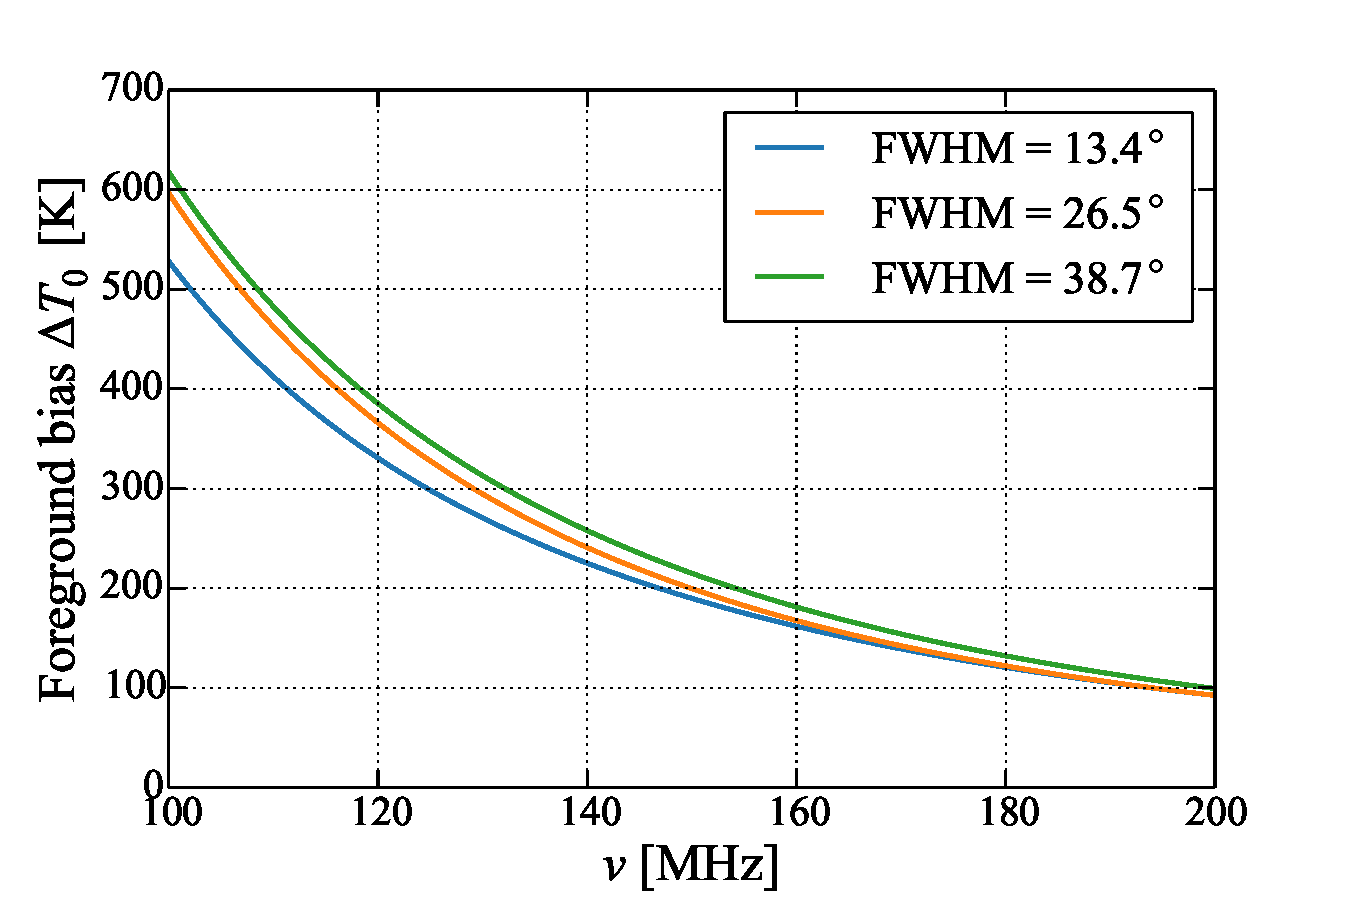
\includegraphics[width=0.50\textwidth]{figures/unsub_T0_beamSize.pdf}
	\caption{\acl{Do this}\mep{What's FWHM?}}
	\label{fig:unsub_T0_beamSize}
\end{figure}

\begin{figure}[h]
	\centering
	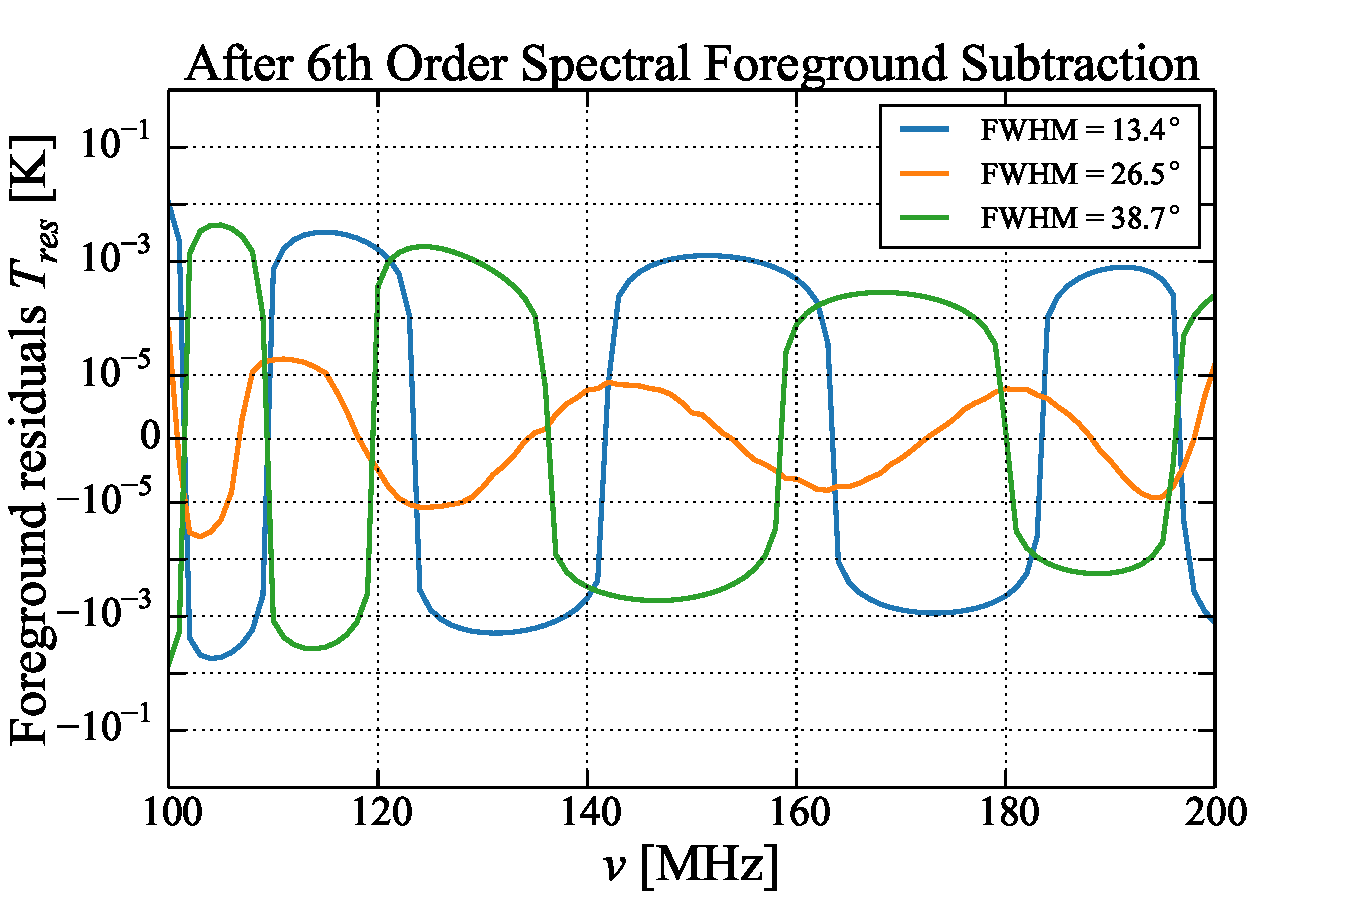
\includegraphics[width=0.50\textwidth]{figures/subPoly6_T0_beamSize.pdf}
	\caption{\acl{Do this}}
	\label{fig:subPoly6_T0_beamSize}
\end{figure}

\begin{figure}[h]
	\centering
	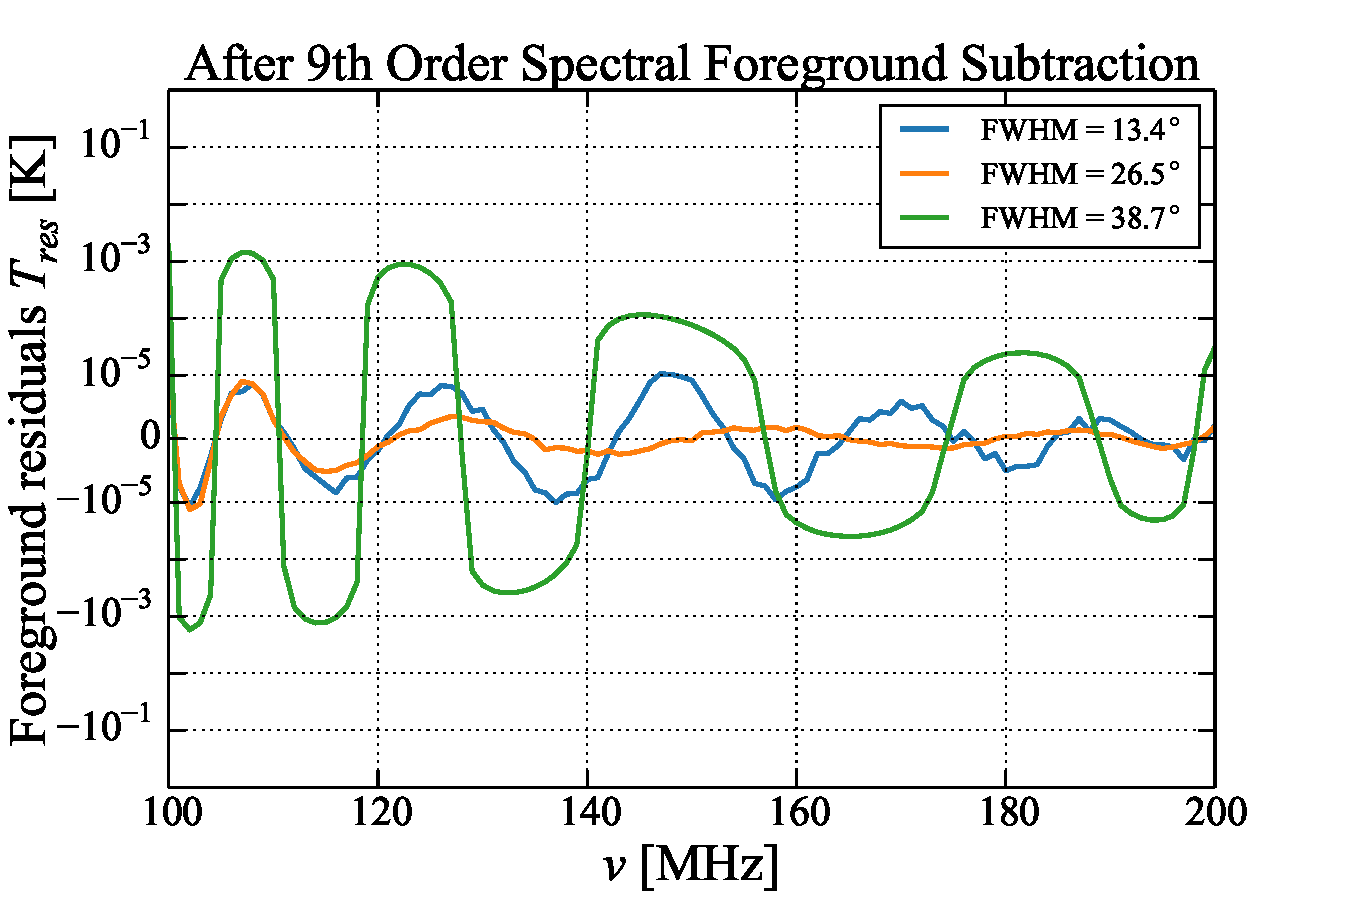
\includegraphics[width=0.50\textwidth]{figures/subPoly9_T0_beamSize.pdf}
	\caption{Same as Figure \ref{fig:subPoly6_T0_beamSize}, but with a $9$th order spectral subtraction. \acl{Add more description}}
	\label{fig:subPoly9_T0_beamSize}
\end{figure}

\acl{Add bl length to plots.}
\acl{Probably want to put in a map of the galaxy somewhere}
\acl{Need to mention somewhere that we're not including the zero mode}
\acl{Insert equation if the non-flat-sky measurement equation hasn't already been written out by this point}xx
\acl{Probably outline earlier the general paradigm we're thinking about}

Yet another consideration in choosing baseline length is instrumental noise. As we have already alluded to, short baselines have greater sensitivity to the spatial monopole of the sky, and therefore have better signal-to-noise. Thus, if one were to add instrumental noise to the preceding discussion, the optimal baseline length would shift towards smaller values (with the primary beam correspondingly increasing in width). Picking a baseline length based on the foregrounds-only analysis of this subsection is therefore in principle sub-optimal. In practice, however, instrumental noise is a sub-dominant contribution to the error budgets of most $21\,\textrm{cm}$ global signal experiments, and the optimal baseline length will only be slightly shorter than the one advocated here. Moreover, since interferometers consist of many baselines, the collective signal-to-noise of an array can compensate for a lower signal-to-noise in any individual baseline, a point that we will explore in the following subsection.

\subsection{How many elements?}
\label{sec:numElems}
Thus far, we have established that the ideal global signal interferometer is one comprised of elements with full-width-half-max primary beam widths of $\sim25^\circ$, packed as closely together as possible. However, we have yet to specify the number of elements. In this section we imagine a regular square grid of $N \times N$ antennas and ask what value of $N$ is required for an interferometer to perform as well as a single dipole in a measurement of the global signal.\acl{Should mention that we're not using the auto-correlation mode} \mep{What's the auto-correlation mode?}

As one adds more and more elements to a regular array (increasing $N$), the main effect is an increase in the number of short baselines, providing repeated measurements of the same visibilities that can be combined to average down instrumental noise. While it is true that adding more elements to an array also gives rise to some longer baselines (since the only way to add antenna elements to a closely packed array is to add them to the periphery), these baselines have minimal response to the global signal and only provide information regarding foregrounds. This information can in principle be used to help with foreground mitigation, but as we shall see when we discuss data analysis in Section \ref{sec:MathForm}, it is difficult to use this information without introducing chromatic signatures into the final global spectrum estimates. It is thus safer to severely downweight the influence of long baselines, minimizing their influence on the final result.

\acl{Gotta switch notations for the covariance below}

With multiple copies of the same baselines, an interferometer can have just as high a signal-to-noise as single dipole experiment, even if each individual baseline is less sensitive to the global signal. To quantify precisely how many such copies are necessary, we will now compute the expected noise variance from our estimator $\widehat{T}_0 (\nu) $ of the global signal. Starting with Equation \eqref{eq:NormedSimpleEst}, we perturb the $j$th visibility $V(\mathbf{b}_j, \nu)$ by adding an additive noise contribution $n_j (\nu)$. Computing the variance $\boldsymbol \Pi(\nu,\nu)$ of the final estimator then gives
\begin{eqnarray}
\boldsymbol \Pi(\nu,\nu) &\equiv& \langle \widehat{T}_0 (\nu)^2 \rangle - \langle  \widehat{T}_0 (\nu) \rangle^2 \nonumber \\
&=&  \frac{\sigma^2}{ \sum_k \big{|} \int  A(\rhat, \nu) \exp\left(i 2\pi \frac{\nu }{c}\mathbf{b}_k \cdot \rhat \right)d\Omega \big{|}^2},
\end{eqnarray}
where we have assumed that the instrumental noise has zero mean, so that $\langle n_j \rangle = 0$. We have additionally assumed that the noise is uncorrelated between baselines, and has a variance of $\sigma^2$, so that $\langle n_i n_j^* \rangle = \sigma^2 \delta_{ij}$. Making the approximation that the sensitivity of the array to the global signal is dominated by the shortest baseline $\mathbf{b}_\textrm{short}$ of which there are $N_\textrm{short}$ copies, the noise variance of an interferometer-estimated global signal reduces to
\begin{equation}
\boldsymbol \Pi(\nu,\nu) \approx \frac{\sigma^2}{ N_\textrm{short} \big{|} \int  A(\rhat, \nu) \exp\left(i 2\pi \frac{\nu }{c}\mathbf{b}_\textrm{short} \cdot \rhat \right)d\Omega \big{|}^2}.
\end{equation}
On the other hand, for a single dipole experiment we have only a single baseline of length zero, so the noise variance is
\begin{equation}
\boldsymbol \Pi(\nu,\nu) = \frac{\sigma^2}{\big{|} \int  A(\rhat, \nu) d\Omega \big{|}^2}.
\end{equation}
Equating these two expression then allows one to solve for the number of short baselines $N_\textrm{short}$ that are needed for an interferometer to have the same thermal noise sensitivity as a single dipole experiment:
\begin{equation}
N_\textrm{short} \approx  \frac{\big{|} \int  A(\rhat, \nu) d\Omega \big{|}^2}{  \big{|} \int  A(\rhat, \nu) \exp\left(i 2\pi \frac{\nu }{c}\mathbf{b}_\textrm{short} \cdot \rhat \right)d\Omega \big{|}^2}.
\end{equation}
To get a rough sense for the magnitude of $N_\textrm{short}$, suppose we make the flat-sky approximation. This gives
\begin{equation}
N_\textrm{short} \approx \frac{\big{|} \widetilde{A}(0)\big{|}^2}{\big{|} \widetilde{A}(\nu \mathbf{b}_\textrm{short} / c)\big{|}^2}.
\end{equation}
For Gaussian beams, we obtain
\begin{equation}
N_\textrm{short} \approx \exp \left( 4 \pi^2 \theta_b^2 \frac{b_\textrm{short}^2}{\lambda^2} \right).
\end{equation}
Now, if one assumes a closely packed array, then $b_\textrm{short}/ \lambda \sim (2\pi \theta_0)^{-1}$. Inserting this into our expression gives $N_\textrm{short} \sim e$. For an $N \times N$ square grid of antennas, there are $N_\textrm{short} = 2(N-1)^2$ shortest baselines formed by adjacent antenna pairs (half of which are in one direction, while the other half are perpendicular) \acl{Phrase this better}. Solving for $N$ then gives $1 + \sqrt{e/2} \approx 2.2$, and therefore even a small array (say, $3\times 3$ or $4\times 4$) will allow an interferometric measurement of the global signal to possess the same thermal noise sensitivity as a signal dipole experiment. \acl{Comment on generalizing this, as well as on how redundancy is not a requirement} \mep{I was just wondering about that -- isn't the redundancy necessary for systematic noise reduction?} \mep{Cool calculation. I really like this section.}


\section{Data analysis choices}
\label{sec:MathForm}
\begin{itemize}
\item How does one actually get from visibilities to a global signal measurement.
\item The error statistics that come for free.
\item Quantification of leakage from other spherical harmonics.
\end{itemize}
\acl{Diagonal normalization is actually minimum-variance solution}

In the previous section, we examined the trade-offs associated with the design of an interferometer targeting the global $21\,\textrm{cm}$ signal. Qualitatively, we concluded that one ought to design an interferometer array with a modest number of antenna elements, packed as closely together as possible. Ideally, the antenna elements should possess primary beams that are neither too narrow nor too broad, with roughly a full-width-half-maximum (FWHM) of $\sim 25^\circ$ \acl{Make sure we consistently quote the same rough number everywhere} for experiments targeting redshifts relevant to reionization.

In this section, we assume that an appropriate array has been constructed, and consider instead various trade-offs in data analysis. Inspired by the near-separable models of \citet{Liu_Switzer_2014}, our proposed analysis methods will usually involve a two-step process. First, the data are analyzed frequency-by-frequency, producing an estimate of the spatial monopole at every frequency channel. Following the per-frequency analysis, the data are combined into a single global signal spectra, where we take advantage of the long frequency-coherence length of foregrounds to perform a final foreground subtraction. In what follows, we will examine the pros and cons of various choices in the detailed implementation of each of these steps.

\subsection{Step 1: Extracting the Spatial Monopole from Visibilities}

We begin with a more general version of Equation \eqref{eq:Vb}, our measurement equation. Discarding the flat-sky approximation, we have
\begin{equation}
V(\mathbf{b}) = \int  T(\mathbf{\hat{r}}) A(\mathbf{\hat{r}}) \exp \left( -i 2 \pi \frac{\nu}{c} \mathbf{b} \cdot \mathbf{\hat{r}} \right) d\Omega,
\end{equation}
where $\mathbf{\hat{r}}$ is a unit vector that specifies locations on the sky. Expressing the sky in terms of spherical harmonics gives
\begin{equation}
\label{eq:VbSphHarm}
V(\mathbf{b}) = \sum_{\ell m} \left(  \int  Y_{\ell m} (\mathbf{\hat{r}}) A(\mathbf{\hat{r}}) e^{ -i 2 \pi \frac{\nu}{c} \mathbf{b} \cdot \mathbf{\hat{r}}} d\Omega \right) a_{\ell m}.
\end{equation}
Since this equation is linear, we may write it as a matrix equation of the form
\begin{equation}
\y = \Q \mathbf{x} + \mathbf{n}
\label{eqn:yQxn}
\end{equation}
where $\y$ is a vector of length $\Nbl$ \acl{Make sure we define this quantity} containing the visibilities measured at different baselines $V(\mathbf{b})$, and we have added a noise contribution $\mathbf{n}$. This noise contribution can be thought of as being comprised of instrumental noise and a ``random" component of unmodeled foregrounds. The matrix $\Q$ is the beam response of an antenna array at different baselines (rows) and different spherical harmonics (columns). Comparing Equations \eqref{eq:VbSphHarm} and \eqref{eqn:yQxn}, we see that the explicit form of $\Q$ is given by 
\begin{equation}
\textrm{Q}_{j,\ell m} = \int d\Omega A(\mathbf{\hat{r}}) Y_{\ell m}(\mathbf{\hat{r}}) e^{-2\pi i \frac{\mathbf{b_\textit{j}}}{\lambda} \cdot \mathbf{\hat{r}}}
\label{eqn:Qdef}
\end{equation}
where $\boldsymbol \theta$ is the angular position on the sky, $A$ is the primary beam for the antennas, $\mathbf{b_{\textit{j}}}$ is the $j$th baseline, and $\lambda$ is the wavelength of observation. The sky is represented by $\mathbf{x}$, which is a vector containing all the spherical harmonic coefficients $a_{\ell m}$. As such, it has length $(\ell_{\textrm{max}}+1)^2$, where $\ell_{\textrm{max}}$ is the largest $\ell$ value used in the model of the true sky. The global signal that we seek is proportional\footnote{Throughout this paper, we adopt a spherical harmonic normalization convention where $Y_{00} (\mathbf{\hat{r}}) = 1/ \sqrt{4\pi}$. A pure monopole $T_0$ then has $a_{00} = \int Y_{00} T_0 d\Omega = \sqrt{4\pi} T_0$, so to recover an estimate of $T_0$ from an estimate of $a_{00}$, one must divide by $\sqrt{4 \pi}$. \acl{Decide if we want to just be a bunch of rebels and define our normalization convention to include the $\sqrt{4\pi}$.}} to the first component of $\mathbf{x}$, i.e., $a_{00}$. Ultimately, then, we only need to form an estimator $\hat{a}_{00}$ of this first component. However, it is crucial to bear in mind that the true $\mathbf{x}$ contains foregrounds with significant power in higher $(\ell, m)$ modes, and that this power may leak into our estimate $\hat{a}_{00}$ of $a_{00}$. The formalism that we present below will provide exactly the right machinery for quantifying such leakage.
%
%The matrix $\Q$ is the beam response of an antenna array at different baselines (rows) and different spherical harmonics (columns). $\Q$ is determined by 
%\begin{equation}
%\textrm{Q}_{j,\ell m} = \int d\Omega A(\boldsymbol \theta) Y_{\ell m}(\boldsymbol \theta) e^{-2\pi i \frac{\mathbf{b_\textit{j}}}{\lambda} \cdot \boldsymbol \theta}
%\label{eqn:Qdef}
%\end{equation}
%where $\boldsymbol \theta$ is the angular position on the sky, $A$ is the primary beam for the antennas, $\mathbf{b_{\textit{j}}}$ is the $j$th baseline, and $\lambda$ is the wavelength of observation. Note that in the formulation of Eqs. \eqref{eqn:yQxn} and \eqref{eqn:Qdef} we assumed that all calculations would be done at a specific frequency. This is not necessary, as we could have expanded the dimensions of Equation \eqref{eqn:yQxn} to include all of the frequencies measured in the experiment. However, we chose to do our calculations for each frequency independently in order to remain conservative in our assumptions about the spectrum.

Since $\Q$ is not in general invertible (or even a square matrix), we cannot solve Equation \eqref{eqn:yQxn} for $\mathbf{x}$ directly and instead can only recover an estimator for $\mathbf{x}$. We consider an estimator of the form 
\begin{equation}
\mathbf{\hat x} = \M \Q^\dagger \Hmat \y,
\label{eqn:xhat}
\end{equation}
where $\Hmat$ and $\M$ are both matrices that can be chosen by the data analyst. The $\Hmat$ matrix is of size $N_\textrm{bl} \times N_\textrm{bl}$, and its role is to encode how the data analyst might wish to weight the different visibilities in forming estimates of the various spherical harmonics. Note that this weighting is in addition to the weighting that is naturally provided by $\Q^\dagger$, which (for a given spherical harmonic mode) upweights baselines if their visibilities are sensitive to that mode and downweights them otherwise. The matrix $\M$ measures $(\ell_\textrm{max} +1)^2 \times (\ell_\textrm{max} +1)^2$, and therefore operates on a set of estimated spherical harmonic modes. Its role is to normalize our estimates of the different modes, and to possibly disentangle them from each other if there is leaked power between the modes. Our choices for $\M$ and $\Hmat$ will determine the statistical properties of our final global signal estimates. For example, the variance $\boldsymbol \Sigma$ of our estimator (the square root of which gives the error bars from instrumental noise) is given by
\begin{equation}
\label{eq:NoiseMatrixSigma}
\boldsymbol \Sigma \equiv \langle \xhat \xhat^\dagger \rangle - \langle \xhat \rangle \langle \xhat \rangle^\dagger = \M \Q^\dagger \mathbf{H} \N \mathbf{H} \Q \M,
\end{equation}
where $\mathbf{N} \equiv \langle \y \y^\dagger \rangle - \langle \y \rangle \langle \y \rangle^\dagger$ is the instrumental noise covariance of the visibilities. This is clearly affected by our choices for $\mathbf{H}$ and $\M$. \acl{Ok, having written things like this, we are committed to using $\mathbf{H}$ instead of $\N$.}

\subsection{A possible choice for $\M$}
\label{sec:badMmatrix}
As a first guess, picking
\begin{equation}
\M = [\Q^\dagger \Hmat \Q]^{-1}.
\label{eqn:M}
\end{equation}
might be considered an attractive choice.
%This form for $\M$ produces an estimator that minimizes $\chi^2 \equiv (\y-\Q \mathbf{\hat x})^\dagger \N^{-1} (\y-\Q \mathbf{\hat x})$. 
The final estimator has the desirable property that its ensemble average $\langle \mathbf{\hat x} \rangle$ satisfies the condition $\langle \mathbf{\hat x} \rangle = \mathbf{x}$. This means that on average, the estimator for a particular spherical harmonic coefficient $\hat{a}_{\ell m}$ is equal to the true coefficient ${a}_{\ell m}$, and there is no leakage between different spherical harmonic modes. An estimate of the monopole is thus truly an estimate of the monopole only, with no contributions from other modes.

However, the $\M$ matrix defined by Equation \eqref{eqn:M} makes an assumption that may not be justified---it assumes that the combination $[\Q^\dagger \Hmat \Q]$ is invertible. Essentially, since the inversion results in $\langle \mathbf{\hat x} \rangle = \mathbf{x}$, we can reverse our line of reasoning to see that any time our observations do not allow different $\hat{a}_{\ell m}$ to be perfectly disentangled from each other, $\Q^\dagger \Hmat \Q$ will be uninvertible. For example, if only part of the sky is surveyed, the best that one can do is to measure linear combinations of different $\hat{a}_{\ell m}$s. Even if the full sky is surveyed (for example by observing the sky with a hypothetical wide-field instrument located at the equator), it is typically difficult to design a broadband instrument that allows for a full inversion without sacrificing the design principles of the previous section, as we will now show.

%\subsection{Balancing physical constraints with information extraction}
%\acl{This is going to be moved to the next section}
%Following the baseline optimization of the previous section, one could in principle substitute our expression for $b_\textrm{opt}$ back into Equation \eqref{eq:DeviationPowGauss} to yield an equation whose only free parameter is the primary beam size $\theta_0$.  Minimizing this equation by varying the beam size then suggests that the beam ought to be made as small as possible.  While this is formally correct for the single baseline case, we will now show that the situation changes somewhat when multiple baselines are involved.
%
%To see why this is so, note that if the beam width $\theta_0$ were made to be small, our earlier assumption that $\widetilde{A}$ is compact no longer applies.  Equation \eqref{eq:PerturbedEst} then implies that our estimator $\widetilde{T}_0$  for the global signal $T_0$ accrues signal from a wide range of modes on the $uv$ plane, particularly since a broad $\widetilde{A}$ allows one the luxury of going to long baselines without sacrificing too much sensitivity to the global signal.\footnote{Alternatively, one can point to Equation \eqref{eq:b_opt} to see that a small $\theta_0$ dictates a long $b_\textrm{opt}$.  However, Equation \eqref{eq:b_opt} must be interpreted with caution in this regime, since its derivation was predicated on a narrow-beam assumption that no longer applies.} In other words, while a long baseline formed from narrow-beam antennas contains much information from the monopole signal, such information is irretrievably mixed in with other spatial modes.
%
%\mep{This intuition makes sense to me, but only because of previous discussions we've had where I've seen a picture of the grids in the uv plane with the different beam sizes mapped out. I doubt that I would have understood what was going on if I hadn't seen that picture. Will there be an image accompanying this discussion, or would others already familiar with the field not need one?}

To perfectly isolate a given spherical harmonic coefficient $a_{\ell m}$ , it is necessary to incorporate information from multiple baselines, each of which measures a slightly different linear combination of spherical harmonics on the sky. A clean extraction requires the data analyst to form yet another linear combination, this time of different visibilities. The goal of this linear combination is to invert the original linear combination of spherical harmonics that was formed by the instrument. Clearly, a necessary condition for this inversion to be successful is for there to be at least as many constraints (i.e., unique visibilities) as there are spherical harmonic coefficients to estimate. Ideally, an array ought to make many independent measurements per spherical harmonic mode to ensure a clean separation of modes.  Since $\ell \sim 2 \pi u$, different $\ell$ modes are separated by $\Delta \ell \sim 2 \pi \Delta u$.  Given that $\ell$ can only take on integer values, this means that having enough measurements is tantamount to requiring our baselines be separated from each other by less than $\Delta u = 1/ 2 \pi$ on the $uv$ plane.  As a concrete example, imagine the square grid of antennas from the previous section, where neighboring antennas separated by a distance $b_\textrm{short}$.  Baselines of this array will also form a square grid of points on the $uv$ plane with the $u$ and $v$ coordinates given by integer multiples of $\Delta u = b_\textrm{short} / \lambda = b_\textrm{short} \nu / c$.  Therefore, in order to have enough measurements for inversion, we must satisfy the condition
\begin{equation}
\label{eq:WantAll}
b_\textrm{short} \ll \frac{c}{2 \pi \nu_\textrm{max}},
\end{equation}
where we have evaluated our constraint at the maximum frequency $\nu_\textrm{max}$ we wish to probe, since that is where it is the most stringent.  On the other hand, as we have argued above, physical constraints on antennas size dictate a spacing satisfying
\begin{equation}
\label{eq:AntSize}
b_\textrm{short} \ge \frac{c}{2 \pi \theta_b \nu_\textrm{min}},
\end{equation}
where this time the tightest constraint occurs at the lowest frequency $\nu_\textrm{min}$. \acl{Comment on how dithering baselines mean that this isn't really an issue if we're trying to measure higher $\ell$. The physical constraints on antenna size only matter if you're trying to access the lowest $\ell$ modes}

The two constraints listed above make it difficult to probe a large frequency range with a single interferometer.  To see this, note that the upper limit on $b_0$ decreases with increasing $\nu_\textrm{max}$, while the lower limit increases with decreasing $\nu_\textrm{min}$.  With a wide enough frequency range, these two limits meet, and to avoid inconsistent constraints, we require
\begin{equation}
\theta_b \ge \frac{\nu_\textrm{max} }{\nu_\textrm{min}}
\end{equation}
as a \emph{minimum} beam size.  Since this critical beam size depends on the ratio of $\nu_\textrm{max}$ to $\nu_\textrm{min}$, it is easier to satisfy our bounds with a narrowband instrument at higher frequencies, which is precisely the scenario that is uninteresting for a global $21\,\textrm{cm}$ signal experiment. Moreover, since $\nu_\textrm{max}$ must be greater than $\nu_\textrm{min}$ the generosity of our bound saturates at $\nu_\textrm{max} = \nu_\textrm{min}$, and our condition then requires that $\theta_0 \ge 1\,\textrm{rad}$. Recalling that $\theta_b$ is the standard deviation of a Gaussian beam (and not the FWHM), we see that essentially one needs horizon-to-horizon beam coverage of the sky. As discussed previously, however, such a beam would be too wide to be optimal, as it would not allow the selective isolation of cold patches in the galaxy. Indeed, one can see from Figure \ref{fig:subPoly9_T0_beamSize} that even with a FWHM of $38.7^\circ$, foreground residuals decrease rather slowly.

\acl{Really need to address the issue of faceting here. Wait, do we?} \mep{What is faceting?}

From this, we see that if one is to adhere to the design principles of Section \ref{sec:BackOfEnvelopeArrayDesign}, the conditions required for $\Q^\dagger \Hmat \Q$ to be invertible will necessarily be violated at some observation frequencies. This problem can be alleviated slightly if one is willing to construct multiple narrowband arrays to collectively cover a wide frequency range. However, this is not only an expensive solution, but also a relatively ineffective one---the best that one can do is to pursue an extreme approach where a different array is constructed (or a single array reconfigured) for every observation frequency, but that corresponds precisely to the $\nu_\textrm{max} = \nu_\textrm{min}$ case discussed above, and we have already seen that the required beam sizes are still to wide.

Alternatively, one may simply replace the inverse of $\Q^\dagger \Hmat \Q$ with its pseudo-inverse whenever the matrix $\Q^\dagger \Hmat \Q$ is uninvertible. In doing so, however, one runs the risk of imprinting sharp spectral features into the final estimate of the global signal. This is because a pseudo-inverse inverts only the modes of a matrix that are present with non-zero eigenvalue, and the set of modes that are present will in general be frequency-dependent. The imprint of sharp spectral features should be avoided at all costs, since sharp features have the ability to masquerade as the cosmological signal.

For all the reasons listed above, we therefore recommend against the use of Equation \eqref{eqn:M} for $\M$. 

\acl{Should probably comment on how the LOFAR paper has violated these conditions in a number of places.}



\subsection{A better choice for $\M$}
\label{sec:BetterM}

As an alternative to Equation \eqref{eqn:M}, consider the diagonal matrix given by 
\begin{equation}
\label{eq:diagM}
\M_{ij} = \frac{\delta_{ij}}{(\Q^\dagger \Hmat \Q)_{ii}}.
\end{equation}
With this choice of $\M$, each $a_{\ell m}$ estimate (each component of $\hat{\mathbf{x}}$) is a linear combination of the true $a_{\ell m}$ coefficients. At first sight, this seems to be a drawback of this choice for $\M$, since our goal is to measure the cosmological monopole. However, we will soon use a variety of illustrative special cases to see that this is not so, and that some leakage between different $a_{\ell m}$ coefficients---if appropriately constrained---is in fact a feature. To quantify this leakage, we take the ensemble average of Equation \eqref{eqn:xhat} and insert Equation \eqref{eqn:yQxn}. This yields
%
%Note that for this choice of $\M$, the ensemble average of $\mathbf{\hat x}$ is $\mathbf{x}$.
%Using this fact, we can directly find the covariance of $\mathbf{\hat x}$ to be 
%\begin{equation}
%\textrm{Cov}(\mathbf{\hat x}) = [\Q^\dagger \N^{-1} \Q]^{-1}
%\label{eqn:Covxhat}
%\end{equation}
%as shown in \citet{Tegmark_CMB_maps_wli}. Therefore, using equation (\ref{eqn:M}) for our statistical analysis allows us to analytically find the error statistics if the noise covariance matrix for the foregrounds and systematics is known. However, since galactic foreground models are not well constrained, it is not safe to assume we know $\N_{\textrm{fg}}$. Consequently, Monte Carlo simulations are still necessary to determine the error bars on measurements analyzed using this method. Note, however, that although we do not know the exact noise covariance $\N$, there is nothing wrong with choosing Equation \eqref{eqn:M} for our data analysis, as long as we do not claim that our error bars are constrained by equation (\ref{eqn:Covxhat}). %-- it just may not be optimal.
%
%Note that two inverses must be taken in order to compute $\M$. In general, $\Q^\dagger \N^{-1} \Q$ will not be invertible, requiring us to approximate the inverse with a pseudo-inverse. We used a pseudo-inverse method that raises the value of the small eigenmodes, inverts, and then projects out those small eigenmodes, as laid out in the appendix of \citet{Tegmark_CMB_spectra_wli}. 
%
%Since $\Q$ is not diagonal, higher spherical harmonic modes will leak into our measurement $\y$. If it were possible to do the inverses in equation \ref{eqn:M}, then these leakages could be dampened down by taking repeated observations to mimic an ensemble average. This is because 
\begin{equation}
\langle \xhat \rangle = \M \Q^\dagger \Hmat \Q \x
\end{equation}
Defining a window function matrix $\W$ as 
\begin{equation}
\W = \M \Q^\dagger \Hmat \Q,
\label{eq:Wform}
\end{equation}
we see that $\langle \xhat \rangle  = \W \mathbf{x}$, so each row of $\W$ gives the linear combination of spherical harmonics actually probed by our estimator $\hat{a}_{\ell m}$. The matrix $\W$ quantifies the amount of leakage between modes, and it depends on both our instrument (via $\Q$) and our data analysis method [via Equations \eqref{eqn:xhat} and \eqref{eq:diagM}]. Of particular interest will be the first row of $\W$, which will tell us what combination of spherical harmonics are actually being measured when we attempt to constrain the monopole $a_{00}$ mode.

The choice of $\M$ used here has several attractive properties. In Appendix \ref{minVarProof} we prove that if $\Hmat$ is used as an inverse noise covariance weighting of visibilities (i.e., if we have $\Hmat = \N^{-1}$), then our diagonal choice for $\M$ minimizes the variance (and therefore the error bars) on $\mathbf{\hat{x}}$. Additionally, Equation \eqref{eq:diagM} has the property that diagonal elements of $\W$ always equal unity, regardless of what $\Hmat$ is used. Focusing on the first row, then, we have $\W_{11} =1$, which implies that the amplitude of a pure monopole sky is preserved by our measurement and data analysis procedures. In other words, there is by construction never any signal loss.
%\acl{Gotta be careful. Our choice is only minimum variance if $\N$ is the noise}\mep{What else would $\N$ be?}\\
%\acl{Talk about normalization as well as the Fisher matrix interpretation}
%
%In order to quantify the relative amount of leakage from the different modes, it is convenient to define
%
%With this definition, the elements of the first row of the window function matrix quantifies the ratios between the contributions from the different modes. A good experimental design would result in a very high ratio between $W_{0,00}$ and all of the other $W_{0,\ell m}$.

\subsubsection{Single Dipole Limit}

Consider the single-dipole limit as an illustrative example of how our choice of $\M$ works, and how leakage between spherical harmonic modes can be a desirable feature. The single-dipole limit is representative of ``traditional" experiments such as EDGES \acl{Maybe we should see if there is a better, more precise descriptor than ``traditional".}\mep{``conventional'', perhaps?}. With a single dipole, the matrix $\mathbf{Q}$ reduces to a single row vector consisting of Equation \eqref{eqn:Qdef} evaluated at baseline length $b_j=0$. The measurement vector $\mathbf{y}$ becomes a single measurement $y$, given by the primary beam integrated over the sky:
\begin{equation}
y = \int T(\mathbf{\hat{r}}) A(\mathbf{\hat{r}}) d\Omega.
\end{equation}
Equations \eqref{eqn:xhat} and \eqref{eq:diagM} then reduce to
\begin{equation}
\mathbf{\hat{x}}_{\ell m} = \frac{\int d\Omega Y_{\ell m} (\mathbf{\hat{r}}) A(\mathbf{\hat{r}})}{\left[ \int d\Omega A(\mathbf{\hat{r}}) \right]^2} y.
\end{equation}
For the global signal (i.e., spatial monopole), we are interested in the first component of this $\mathbf{\hat{x}}$ vector. Isolating this and dividing both sides $\sqrt{4\pi}$ to convert from our $a_{00}$ to the all-sky average, we obtain
\begin{equation}
\label{eq:singleElementExtraction}
\widehat{T}_0 = \frac{y}{ \int d\Omega A(\mathbf{\hat{r}}) },
\end{equation}
which is the estimator that one would have guessed from simple considerations---the measurement $y$ is just a weighted average of the sky, and the denominator normalizes the weights. This is in fact also a special case of the estimator given in Equation \eqref{eq:singleBlSillyEst}, where the baseline vector $\mathbf{b}$ is set to zero. Note that there was no need to specify the matrix $\Hmat$, because with only a single measurement from a single dipole, $\Hmat$ reduces to a single scalar. The copy of $\Hmat$ in Equation \eqref{eqn:xhat} will therefore always cancel the copy in \eqref{eq:diagM}.
%
%Note that we did not have to specify a form for the noise covariance $\mathbf{N}$. With a single dipole experiment, our measurement consists of a single number, so $\mathbf{N}$ becomes a single scalar and the factor of $\mathbf{N}^{-1}$ in Equation \eqref{eqn:xhat} is always canceled out by the one appearing in Equation \eqref{eq:diagM}. This is a limitation of single dipole experiments. With the instrument having performed an irreversible spatial averaging over the sky, we lose the ability to judiciously downweight low signal-to-noise and/or foreground systematics-dominated data.

Explicitly evaluating Equation \eqref{eq:Wform} for our single dipole case, the window function for the sky monopole (i.e., the first row of $\W$) is given by
\begin{equation}
\W_{0}(\ell,m) = \frac{\int d\Omega A(\mathbf{\hat{r}}) Y_{\ell m} (\mathbf{\hat{r}})}{\int d\Omega A(\mathbf{\hat{r}}) / \sqrt{4 \pi}}.
\label{eq:singleDipoleW0}
\end{equation}
Naively, one might have hoped for $W_0$ to be zero for all values of $\ell$ and $m$ except for $(\ell, m) = (0,0)$, so that our estimator for the sky monopole does not contain any leaked power from other spherical harmonics. This is what the $\M$ matrix of Section \ref{sec:badMmatrix} would have achieved, and is what was sacrificed by our new choice of $\M$. On closer examination, however, the leakage appears to be rather innocuous, and is simply the result of our having only surveyed a small portion of the sky (the part that lies within the primary beam). Confirming this interpretation is the form of the numerator in Equation \eqref{eq:singleDipoleW0}, which is the spherical harmonic decomposition of the primary beam.

As discussed above in Section \ref{sec:BackOfEnvelopeArrayDesign}, it is advantageous to concentrate observations on cooler parts of the sky. The non-zero width of the window function given by Equation \eqref{eq:singleDipoleW0} is thus a desirable feature. Another way to see this is to recognize that focusing on a small patch of the sky (and therefore accepting our broader window function) gives us a better estimate of the \emph{cosmological} monopole signal than if we were somehow able to force the window function to be zero away from $(\ell,m) = (0,0)$. In the latter case we would be better estimating the monopole signal of total sky emission, but much of this would be due to the foreground contribution. The key point is that the foregrounds also have a monopole, and without an \emph{a priori} way to distinguish between the monopole of the cosmological and the monopole of the foregrounds, making a ``clean" measurement of the sky's monopole simply adds stronger foregrounds.

\subsubsection{Multi-baseline case}

We now turn to the multi-baseline case. With our measurement $\mathbf{y}$ now consisting of more than just a single number, there is the opportunity to weight our data in non-trivial ways. Put another way, it will be necessary to decide on a form for $\Hmat$, since its two copies will no longer cancel when forming $\xhat$.

Consider an inverse noise covariance weighting of $\Hmat = \mathbf{N}^{-1}$. With the assumption that instrumental noise is uncorrelated and uniform across different baselines, this is equivalent to $\Hmat = \mathbf{I}$. The window function matrix then simplifies to $\W \propto \M \Q^\dagger \Q$, with the key piece being $\Q^\dagger \Q$. The $\M$ matrix is irrelevant to any discussion of leakage between different spherical harmonics, since the form given by Equation \eqref{eq:diagM} is diagonal, and thus the matrix only provides a normalization for each spherical harmonic without further mixing between modes. Evaluating the window function matrix explicitly, we obtain
\begin{eqnarray}
\W_{\ell m, \ell^\prime m^\prime} &\propto& \left( \Q^\dagger \Q \right)_{\ell m, \ell^\prime m^\prime} \nonumber \\
& \propto & \sum_k \left( \int d\Omega A(\rhat) Y^*_{\ell m}(\rhat) e^{i 2 \pi \frac{\mathbf{b}_k}{\lambda} \cdot \rhat }\right) \nonumber \\
&& \times \left( \int d\Omega^\prime A(\rhat^\prime) Y_{\ell^\prime m^\prime}(\rhat) e^{-i 2 \pi \frac{\mathbf{b}_k}{\lambda} \cdot \rhat^\prime }\right).
\end{eqnarray}
For the purposes of measuring the global signal, it is again the first row of this matrix that is the most relevant. Making the flat-sky approximation for the sake of intuition yields
\begin{equation}
\label{eq:AnotherApproxWindow}
\W_{0}(\mathbf{u}) \propto \sum_k \widetilde{A}^* \left( \frac{\mathbf{b}_k}{\lambda} \right) \widetilde{A} \left( \mathbf{u} - \frac{\mathbf{b}_k}{\lambda} \right).
\end{equation}
Now, $\widetilde{A}$ is a function that peaks at the origin and drops off on a characteristic scale $(2 \pi \theta_b)^{-1}$. Thus, this expression tells us that the highest $u = | \mathbf{u} |$ scale that is probed by our global signal interferometer is
\begin{equation}
u \sim \frac{b_\textrm{max}}{\lambda} + \frac{1}{2 \pi \theta_b} = \frac{N\sqrt{2} +1}{2 \pi \theta_b},
\end{equation}
where $b_\textrm{max}$ is the longest baseline in the array, and in the last equality we assumed a closely packed $N \times N$ square array, just as we did in Section \ref{sec:numElems}. The reciprocal of this expression gives the finest angular scale $\theta_\textrm{fine}$ that our interferometer is sensitive to:
\begin{equation}
\theta_\textrm{fine} \sim 9^\circ \left( \frac{\textrm{FWHM}}{26.5^\circ} \right) \left( \frac{N \sqrt{2} + 1}{5 \sqrt{2} + 1} \right)^{-1}.
\end{equation}
Here, we have eliminated $\theta_b$ (which corresponds to the standard deviation for a Gaussian beam) in favor of the FWHM, and have used a fiducial array size of $N=5$ to be slightly on the conservative side of our optimal $N=3$ or $4$ from Section \ref{sec:numElems}. We may thus conclude that an interferometer that is designed in accordance with the principles laid out in Section \ref{sec:BackOfEnvelopeArrayDesign} will not be sensitive to scales finer than $\sim 10^\circ$. Since the anisotropies of the cosmological $21\,\textrm{cm}$ signal are negligible beyond a scale of $\sim 1^\circ$ to $2^\circ$ \acl{Cite the Bittner \& Loeb paper}, the modes that are measured by our interferometer are essentially global signal modes, even if they are not formally the $\mathbf{u} = 0$ (or $\ell = m = 0$) mode. Indeed, this argument is one that is implicitly invoked by most theoretical simulations of the global signal---since full sky simulations are too computationally expensive to perform, most (if not all) simulations simply average over an angular field of view that is much greater than the angular scale of anisotropies, and declare the result the global signal.
% \acl{Point out that this is actually a conservative estimate. In practice one might be able to build out larger, because the longer baselines are downweighted by the first factor of A-tilde.}

In short, the leakage of higher spherical harmonic modes into our estimate of the global signal is likely not a concern. In fact, our estimate is a conservative one, because we assumed that the longest baseline of an array contributes significantly to the estimator of the monopole mode. In practice, long baselines have so little response to the monopole that its contribution to our estimator is heavily downweighted by the presence of $\mathbf{Q}^\dagger$. This manifests itself as the $\widetilde{A}^* ( \mathbf{b}_k / \lambda )$ term in our approximate window function, Equation \eqref{eq:AnotherApproxWindow}. The window function for the monopole is therefore preferentially dominated by the baselines that probe broad angular scales.

Importantly, however, our argument relied on the fall-off of $\widetilde{A}$. If the primary beam contains fine features, $\widetilde{A}$ becomes a rather broad function, and one's interferometer begins to be sensitive to the more substantial small-scale modes of the $21\,\textrm{cm}$ anisotropies. This may be an important effect for the global signal measurements performed at LOFAR using lunar occultations, which imprints small spatial structures in the beam \acl{Cite Harish's paper}. Fortunately, our formalism provides an easy way to compute the relevant window functions to assess the viability of occultation measurements.

%\acl{We could extend this section to make it more imaging-centric, but it's probably not worth it} \mep{I like it as-is. Going into imaging would be a distraction.}
%
%\acl{Make the point that because we have a single measurement, the noise covariance always drops out. We can't really do anything to weight}
%
%
%
%\acl{Should probably also include stuff about window function normalization}
%\acl{Also don't forget to mention how $\N$ is regularized}
%
%\mep{Figure time! Show the green/pink plots of 1st row of window function for different arrays.}
%\acl{I'm wondering if it might actually be good to display the window function plots in a way that's averaged over $m$, since for a given $\ell$ the $m$ value basically just changes the direction.  One could imagine something analogous to the angular power spectrum, which is often estimated by computing $\hat{C}_\ell = \frac{1}{2\ell + 1} \sum_{m=-\ell}^{\ell} |a_{\ell m}|^2$.  We could do an analogous sum.  On the other hand, the baseline vector breaks the symmetry and does pick out a direction.  So if we want to build that intuition, it could be useful to show the different $m$ values separately.}
%
%\begin{figure}[h]
%	\centering
%	%\includegraphics[width=0.55\textwidth]{figures/oldFigures/W_matrix_filler.pdf}
%	\caption{\mep{Of course, this will have to be updated when the new data comes in. Probably to show several figures for different arrays?}\mep{Uh.... Weird stuff happens if I try to make the figure bigger. It's not wrapping the text and is trying to keep the figure in the column somehow?? Not sure what's up with the formatting style here.}\acl{Is this better? Or did you actually want to make this a figure that spans both columns? If so, change ``figure" to ``figure*" when you do \textbackslash begin.}}
%	\label{fig:WindowFunction}
%\end{figure}
%
%\acl{The tone of the writing is excellent, btw.}



%
%\section{Exploration of arrays}
%\begin{itemize}
%\item Show plots of different arrays that we tried.
%\item (Maybe spherical harmonic plots with fringe patterns overlaid on spherical harmonics).
%\item Reasoning behind our crazier-looking arrays.
%\item Rules of thumb for designing a global signal interferometer.
%\end{itemize}

\subsection{Choices for $\Hmat$}

Having motivated our diagonal choice for $\M$, we now consider our choice for $\Hmat$, which weights the visibilities. We will find that although the presence of $\Hmat$ in our estimator provides additional flexibility that can in principle be harnessed to better suppress foregrounds, a ``simple is best" approach of setting $\Hmat = \mathbf{I}$ is more robust and gives better final results.

To see how $\Hmat$ can aid in foreground mitigation, imagine we were able to accurately model the full covariance matrix of foregrounds $\mathbf{N}_\textrm{fg}$. Picking $\Hmat = \Nfg^{-1}$ in Equation \eqref{eqn:xhat} would then downweight select modes in the visibilities $\y$ that are particularly foreground-contaminated, before the $\Q^\dagger$ matrix converts the collection of visibilities into estimates of spherical harmonic estimates (albeit unnormalized ones, prior to the action of $\M$). In practice, one does not possess sufficient information to construct a full covariance matrix, and approximations must be made.

Suppose that one were to approximate the foreground covariance matrix as diagonal in some judiciously chosen basis. Of course, any matrix is by construction diagonal in its own eigenbasis. However, moving into this basis would require knowing the exact covariance matrix to begin with. Instead, our goal should be to find some basis that sufficiently captures the features of the matrix that are needed for foreground mitigation. Consider, for example, a matrix that is diagonal in harmonic space. Modeling the foreground sky in such a way is tantamount to saying that the foregrounds are statistically isotropic, and therefore describable using a power spectrum. While this may be sufficient for some applications, in our case it is relatively unhelpful. To see this, consider the action of an interferometer in the flat-sky approximation.  Disregarding the primary beam for a moment, each baseline would simply measure a different Fourier mode of the sky. In the full formalism, $\Q$ maps spherical harmonics to visibilities; in the flat-sky approximation, the spherical harmonics and visibilities both reduce to Fourier modes, so $\Q$ correspondingly reduces to $\mathbf{I}$. The $\M$ matrix in our estimator therefore simplifies to $\Hmat^{-1}$, which then acts directly on our $\Hmat$ weighting of the visibilities (since $\Q^\dagger$ is now the identity). The two copies of $\Hmat$ then cancel each other, and the estimator becomes $\xhat = \y$. Conceptually, the visibilities are already a measurement of the harmonics of the sky, and thus the different visibilities never have to mix with each other to produce our final (harmonic) estimator. Any downweighting of a strong foreground mode in harmonic space is then simply upweighted back to its original strength, and no foreground mitigation happens. Of course, in a realistic situation we violate the assumptions of the flat-sky and a uniform primary beam, but the foreground suppression effects are still likely to be minimal.

In contrast, consider a foreground covariance matrix that is diagonal---but not the identity---in image space. When transformed into visibility space, the $\Nfg$ matrix then contains off-diagonal elements. In acting on $\y$ through $\Hmat = \Nfg^{-1}$, different visibilities are then mixed together in an effort to suppress foregrounds. Physically, this corresponds to the statement that if the foregrounds are not statistically isotropic (so that the diagonal elements of the covariance vary), the harmonic coefficients of the sky will end up possessing correlated phases. Since the visibilities are approximately measurements of the harmonic sky, they too will be correlated. These correlations can then be used to downweight the contributions of brighter parts of the foreground sky.

Concretely, suppose we form an image-space covariance matrix $\R$, which is given by
\begin{equation}
\label{eq:Rmatrix}
\R_{ij} = m^2(\rhat_i) \delta_{ij}
\end{equation}
where $m^2(\rhat_i)$ is the model for the foreground sky brightness at the $i$th pixel, with angular position $\rhat_i$. To use this in our estimator then requires translating this matrix into visibility space by constructing
\begin{equation}
\label{eq:GRG}
\Nfg = \mathbf{G} \R \mathbf{G}^\dagger,
\end{equation}
where
\begin{equation}
\mathbf{G}_{ij} = A(\rhat_j)\exp\left(-i2\pi \frac{\mathbf{b_\textit{i}}}{\lambda} \cdot \boldsymbol \rhat_j\right) \Delta \Omega,
\end{equation}
with $\Delta \Omega$ being the solid angle encompassed by each pixel of our sky model. Note that in general $\Nfg$ is a smaller matrix than $\R$, since the former measures $N_\textrm{bl} \times N_\textrm{bl}$ while the latter measures $N_\textrm{pix} \times N_\textrm{pix}$, where $N_\textrm{pix}$ is the number of pixels in our model.

In Figure \ref{fig:Ncomparison}, we compare the global signal estimators that result from analyzing simulated data using $\Hmat = \Nfg^{-1}$ to those that are obtained with $\Hmat = \mathbf{I}$. For the foreground model in Equation \eqref{eq:Rmatrix}, we use the Haslam map at $408\,\textrm{MHz}$. Note that even though the Haslam map will have the wrong amplitude for observations in our frequency band, the overall amplitude of our foreground map will always cancel out in our final estimator, since $\Hmat$ appears both in Equation \eqref{eqn:xhat} and our normalization $\M$. In other words, only the angular \emph{shape} of the foreground sky matters. The instrumental simulations used for Figure \ref{fig:Ncomparison} are identical to those of Section \ref{sec:beamSize}, except with the FWHM of the primary beams set to $88^\circ$. With a broader beam, one exaggerates the effect of setting $\Hmat = \Nfg^{-1}$. This is because a larger field of view captures more of the strongly anisotropic nature of foregrounds, which makes a selective downweighting of the brighter parts of the sky more important. Figure \ref{fig:Ncomparison} shows that such a downweighting does in fact reduce the brightness of the foregrounds, but only by a small amount. We find that the reduction is more pronounced if observations are centered on the galactic plane. There, the foregrounds vary strongly with galactic latitude, making downweightings much more important, and reductions of up to a factor of $\sim 2$ are possible. In practice, however, one tends to avoid observing in the galactic plane anyway. Therefore, the benefits of $\Hmat = \Nfg^{-1}$ are likely to be minimal, particularly when one moves back to using narrower beams suggested in Section \ref{sec:beamSize}, which can more easily isolate patches of the sky that are more approximately isotropic.

\begin{figure}[h]
	\centering
	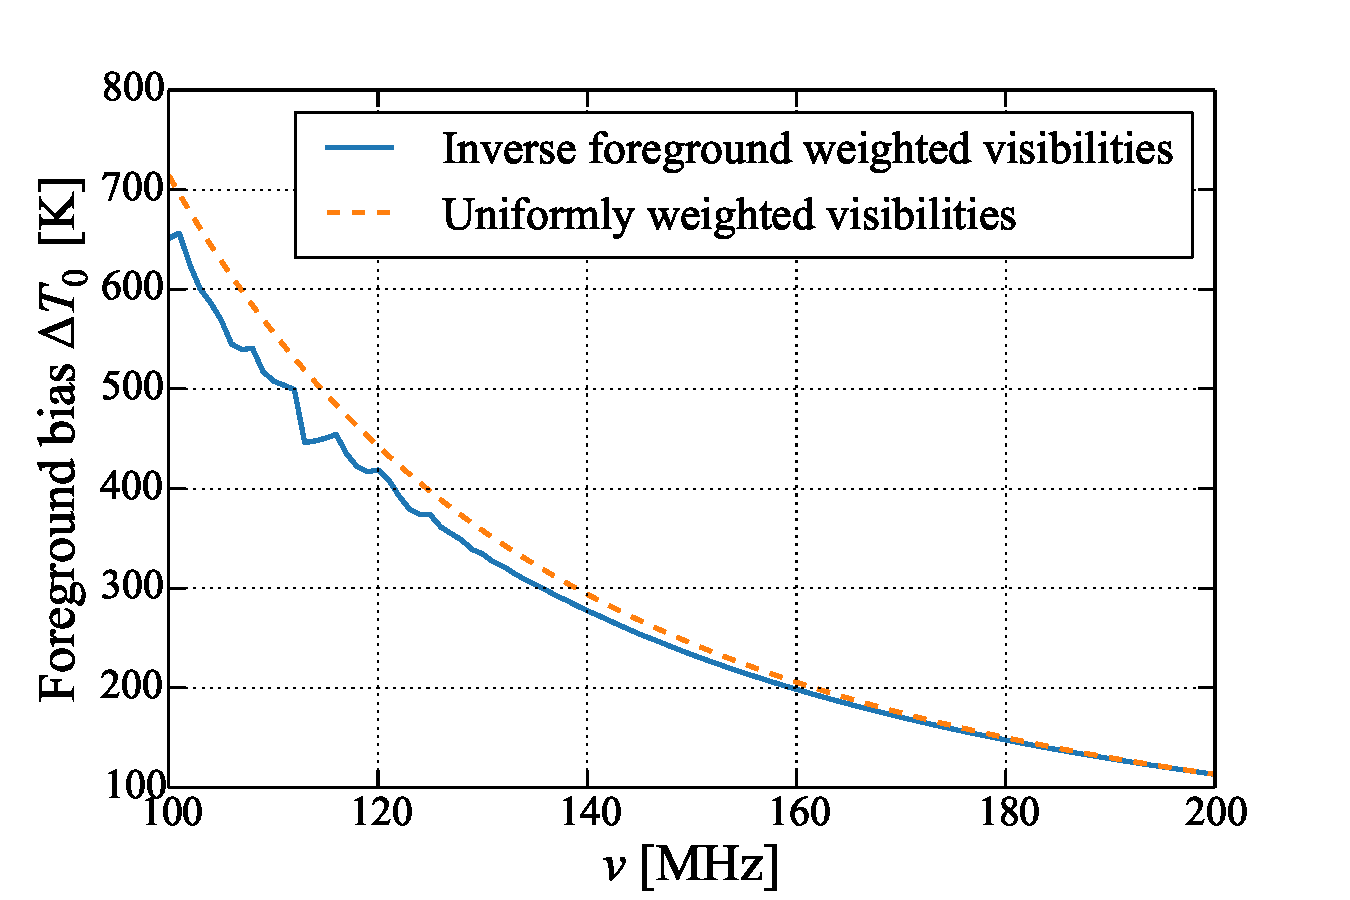
\includegraphics[width=0.50\textwidth]{figures/Ncomparison.pdf}
	\caption{\acl{Do this}}
	\label{fig:Ncomparison}
\end{figure}

More seriously, setting $\Hmat = \Nfg^{-1}$ has the potential to introduce harmful artifacts into the final spectra. For example, bumpy spectral features are clearly visible in Figure \ref{fig:Ncomparison}, which can easily be confused with true spectral features in the cosmological signal. We find that such unsmooth structures are reasonably generic with this choice of $\Hmat$. Much of this is because the quest to downweight brighter portions of the foreground sky requires the isolation of spatially small patches. To isolate these patches, high angular resolution is necessary, which means that the estimator must weight longer---and more chromatic---baselines more heavily. Long baselines also have the disadvantage of having low sensitivity to the monopole. With a heavier weighting of long baselines, it is more difficult for an interferometer to match the thermal noise sensitivity of a single dipole experiment. \acl{Why do we keep calling it a single dipole experiment? Single element would be better} Although in future work it may be possible to eliminate all of these issues with a more sophisticated foreground-motivated form of $\Nfg$, for now we propose the use of $\Hmat = \mathbf{I}$.

\subsection{Step 2: Fitting smooth foregrounds}
\label{sec:fitting}
After the frequency-by-frequency combination of visibilities into an initial estimate of the monopole mode, one obtains spectra such as those shown in Figure \ref{fig:unsub_T0_beamSize} and Figure \ref{fig:Ncomparison}. The spectra are clearly still dominated by smooth, near-power law foregrounds. It is therefore necessary to take further steps to mitigate foregrounds once the data have been reduced to a single spectrum.

One approach is to subtract off smooth functions from the spectrum, be they polynomials or more data-driven forms (such as principal component spectra used in \acl{Cite Eric and I}). The (hopefully foreground-free) residuals can then be compared to theoretical models for the global signal, although care must be taken to properly account for the possibility that part of the cosmological signal may have been subtracted along with the foregrounds. An alternate approach, which we adopt in the rest of this paper, is to follow in the footsteps of \acl{Cite DARE, Jonathan, and Bernardi et. al.} and to fit for foreground and cosmological model parameters simultaneously. Doing so provides a natural description for signal loss, which manifests itself as degeneracies between foreground parameters and cosmological model parameters. One important trade-off is to decide how many foreground parameters to include. If too many parameters are used, much of the cosmological signal will be absorbed into the foreground model, resulting in large degeneracies and large final error bars on the parameters. On the other hand, having too few parameters will result in foreground residuals that will bias cosmological parameter values. We take the same approach as \acl{Cite Bernardi et al.}, where we include just enough foreground parameters for the cosmological parameter bias to be subdominant to the errors.

\subsection{Summary of data analysis methods}

In summary, we propose a ``simple is best" approach for extracting the global signal from interferometric data. In what follows, we will set $\Hmat = \mathbf{I}$ and adopt Equation \eqref{eq:diagM} for $\M$. Plugging these into Equation \eqref{eqn:xhat}, recasting our vector/matrix expressions in terms of continuous functions, we obtain
\begin{equation}
\label{eq:IntegralEstInterferometer}
\widehat{T}_0 (\nu)= \frac{\sum_j \left[ \int d\Omega A(\rhat, \nu) \exp\left( i 2 \pi \frac{\nu }{c} \mathbf{b}_j \cdot \rhat \right)\right] V(\mathbf{b}_j, \nu)}{\sum_k \big{|} \int d\Omega A(\rhat, \nu) \exp\left( i 2 \pi \frac{\nu }{c} \mathbf{b}_k \cdot \rhat \right) \big{|}^2},
\end{equation}
where we have re-introduced the frequency-dependence of various quantities in our notation. Essentially, our estimator amounts to performing a linear fit (frequency-by-frequency) to our data in order to find the value of the monopole that is most consistent with our measured visibility. Following this, we fit the spectrum with a model that includes foreground fits and cosmological parameters. For our foreground fits, we use the same parametric forms as we did in Section \ref{sec:beamSize}, namely Legendre polynomials in $\log \widehat{T}$-$\log \nu$.

\acl{Talk about how it doesn't really matter how many spherical harmonic coefficients one solves for. Maybe?}


%\section{Set-up of numerical studies}
%\acl{Be sure to include a formula for noise}
%In the following section, we will 




%
%\section{Foregrounds and their mitigation}
%\label{sec:Foregrounds}
%\begin{itemize}
%\item General characteristics of foregrounds.
%\item Desire to avoid using too much spectral information because the signal itself is a spectrum.
%\item How to use angular information.
%\item (Modifications to array design to account for foregrounds).
%\end{itemize}
%
%The primary source of contamination in a global signal experiment comes from galactic foregrounds, which make extraction of the global signal difficult for a number of reasons. Primarily, the galactic foregrounds are many orders of magnitude brighter than our expected signal, so finding the global signal through a simple spatial average over the sky would result in a measurement dominated by foregrounds. Also, since both the galactic foregrounds and the expected global re-ionization signal are spectrally smooth, foreground subtraction techniques will likely be unreliable. Therefore, we propose using angular information to differentiate galactic foregrounds from the global signal. 
%
%In order to best remove the foregrounds from our data, we construct a noise covariance matrix for the foregrounds: $\Nfg$. $\Nfg$  shows the correlation between the Fourier modes probed by the antenna array, and hence has dimensions $\Nbl \times \Nbl$. One method \mep{Are there other methods?} to generate $\Nfg$ from a model of the sky is to first find a covariance matrix of the sky $\R$ and transform that matrix into the Fourier domain of the visibilities via the matrix transformation 
%
%\begin{equation}
%\Nfg = \mathbf{G} \R \mathbf{G}^\dagger
%\label{eqn:Nfg}
%\end{equation}
%Since $\R$ has dimensions $N_{\textrm{pix}} \times N_{\textrm{pix}}$, note that $\mathbf{G}$ must have dimensions $\Nbl \times N_{\textrm{pix}}$. Although $\mathbf{G}$ serves a purpose similar to a Fourier transformation matrix, it is not precisely a Fourier matrix as that would probe every single possible Fourier mode, and we only want those that correspond to our array's baselines. As such, $\mathbf{G}$ is defined by 
%\begin{equation}
%G_{i,j} = A(\rhat_j)e^{-2\pi i \frac{\mathbf{b_\textit{i}}}{\lambda} \cdot \boldsymbol \rhat_j} \Delta \Omega
%\end{equation}
%where $\rhat_j$ is the angular position of the $j$th pixel,  $\Delta \Omega$ is the solid angle encompassed by each pixel, and $\mathbf{b_\textit{i}}$ is the $i$th baseline. 
%
%\mep{Insert here stuff on how you're calculating $\R$?}
%
%Once $\mathbf{G}$ has been found, all that remains is to find the covariance in the image space: $\R$. A naive model for the image covariance would be to create a diagonal matrix defined by 
%\begin{equation}
%\R_{i,i} = m^2(\rhat_i)
%\end{equation}
%where $m^2(\rhat_i)$ is the brightness of the sky \mep{Is this true?} at the pixel with angular position $\rhat_i$. This model can be useful because it ensures that there will be non-diagonal correlations in the spherical harmonic space and because it makes equation (\ref{eqn:Nfg}) easy to compute. However, a diagonal covariance is not a realistic portrayal of the true sky, since each pixel is clearly correlated to the ones near it. 
%
%At the other extreme, 
%
%\acl{An interesting point I just realized.  We can make the argument that since the normalization of $\mathbf{N}$ scales out of the expression for $\hat{\mathbf{x}}$, our foreground mitigation scheme is a very conservative one that only uses shape information, and not the detailed spectral form of our foreground model.}
%\acl{Somewhere, we also need to address rotation synthesis}
%\acl{Also need to add noise to simulations}.

\section{Numerical simulations}
\label{sec:SimResults}

In this section, we bring together the various lessons that we have learned regarding instrument design and data analysis to numerically forecast the performance of a fiducial global signal interferometer. Much of our simulation methodology has already been employed in previous sections to produce intermediate results, but we will provide a quick summary here (and add new details) for the reader's convenience.

Guided by the rough arguments of Section \ref{sec:BackOfEnvelopeArrayDesign}, we simulate visibilities from a $5\times5$ square grid of tightly packed antennas. The primary beam of each element is taken to be a tapered Gaussian of the form given by Equation \eqref{eq:TaperedGauss}, with $\theta_b = 0.2\,\textrm{rad}$ (for a FWHM of $26.5^\circ$). \acl{Talk about beam evolution} We assume that observations are centered on the Northern Galactic Pole and span a band consisting of $1\,\textrm{MHz}$ channels from $100\,\textrm{MHz}$ to $200\,\textrm{MHz}$. For comparison, we also predict the performance of a single-element global signal experiment using the same type of antenna element and the same observing strategy.

For our simulated foreground sky, we use the same set-up as we did in Section \ref{sec:beamSize}, where each pixel of the $408\,\textrm{MHz}$ map is extrapolated to the relevant frequencies on a pixel-by-pixel basis using Equation \eqref{eq:HaslamExtrap}. The parameters in the power-law-like extrapolation are drawn randomly as before, and we generate $10,000$ different realizations of the foreground sky. With each sky, we then simulate visibilities and total power measurements for the interferometric and single element measurements, respectively. Frequency-by-frequency estimates are of the global signal are then obtained using Equation \eqref{eq:singleElementExtraction} for the single element and Equation \eqref{eq:IntegralEstInterferometer} for the interferometer. The results are then averaged together to yield mean foreground spectra for each type of experiment. Finally, smooth foreground components are fit from these spectra in the manner described in Sections \ref{sec:beamSize} and \ref{sec:fitting}. The result is a set of residual foreground spectra.

Aside from residual foregrounds, our forecasts must also incorporate instrumental noise. Modeling this contribution requires three separate covariance matrices. The first is the instrumental noise covariance $\N$ of the visibilities. We assume that the instrumental noise is uncorrelated between different baselines, so that\footnote{Note that our expression differs from the standard radiometer equation by a factor of $\Omega_p$ because we have adopted an unusual convention where our visibilities have units of temperature times solid angle\acl{Instead of the usual...}}
\begin{equation}
\N_{ij} (\nu) = \frac{T^2_\textrm{sys}(\nu) \Omega_p}{t_\textrm{int} \Delta \nu} \delta_{ij},
\end{equation}
where the indices refer to different baselines, $\Omega_p = \int  A(\mathbf{\hat{r}}) d\Omega$ is the size of the primary beam, $T_\textrm{sys}$ is the system temperature, $\Delta \nu$ is the channel width, and $t_\textrm{int}$ is the total integration time. We take $\Delta \nu = 1\,\textrm{MHz}$ and $t_\textrm{int} = 300\,\textrm{hrs}$. For the system temperature we assume that the measurements are sky-noise dominated, and we set $T_\textrm{sys}$ equal to the primary beam averaged sky temperature.

With the noise covariance of the visibilities $\N$ in hand, we can obtain the covariance matrix $\boldsymbol \Sigma$ of our estimator $\xhat$. To do so, we insert $\N$ into Equation \eqref{eq:NoiseMatrixSigma}. Since $\xhat$ contains estimates of all the spherical harmonic modes that we wish to solve for,   it is an $(\ell_\textrm{max} +1)^2 \times (\ell_\textrm{max}+1)^2$ matrix relating all the errors on the $a_{\ell m}$ estimates to one another. With our focus being the monopole term, we require only the first element on the diagonal of $\boldsymbol \Sigma$. Extracting this element for every observation frequency, we can place the resulting variances along the diagonal of yet another covariance matrix $\boldsymbol \Pi$. This is the frequency-frequency noise covariance matrix of our final spectrum, and by populating only its diagonal elements (setting all other elements to zero), we are assuming that noise contributions from different frequencies are uncorrelated. Note that in the case of the single element experiment, the diagonals of $\boldsymbol \Pi$ reduce to $T^2_\textrm{sys}(\nu) \Omega_p / t_\textrm{int} \Delta \nu$, as one might expect.

\acl{Add comment about rotation synthesis, as well as why we're allowed to average of MCs}

With a final noise covariance and a residual foreground spectrum on hand, we can translate our 

To evaluate the effectiveness of our global signal interferometer, we employ a Fisher matrix formalism. Our set-up is essentially identical to that of \acl{Cite Gianni et al.}, and thus we relegate a review of the formalism to Appendix \ref{fisher}. As a toy model for the dark ages, we again follow \acl{Cite Gianni et al.} and model the dip at $\sim 70\,\textrm{MHz}$ as a Gaussian:
\begin{equation}
\label{eq:Dip}
T_\textrm{dip}(\nu) = -A \textrm{exp}\left ( -\frac{(\nu - \nu_0)^2}{2\sigma^2} \right ),
\end{equation}
where $A$ is the amplitude of the signal, $\nu_0$ is the center of the pre-reionization absorption dip, and $\sigma$ is the width. For the reionization signal, we use the form
\begin{equation}
\label{eq:Step}
T_\textrm{reion}(\nu) = \frac{T_{21}}{2} \sqrt{\frac{1+z}{10}}\left[ 1 +  \tanh \left( \frac{z-z_r}{\Delta z} \right)\right],
\end{equation}
where $z_r$ is the redshift of the mid-point of reionization, $\Delta z$ is its rough duration, $T_{21}$ is an overall amplitude, and $z = (1420 \,\textrm{MHz} / \nu) - 1$.

\begin{figure}[h]
	\centering
	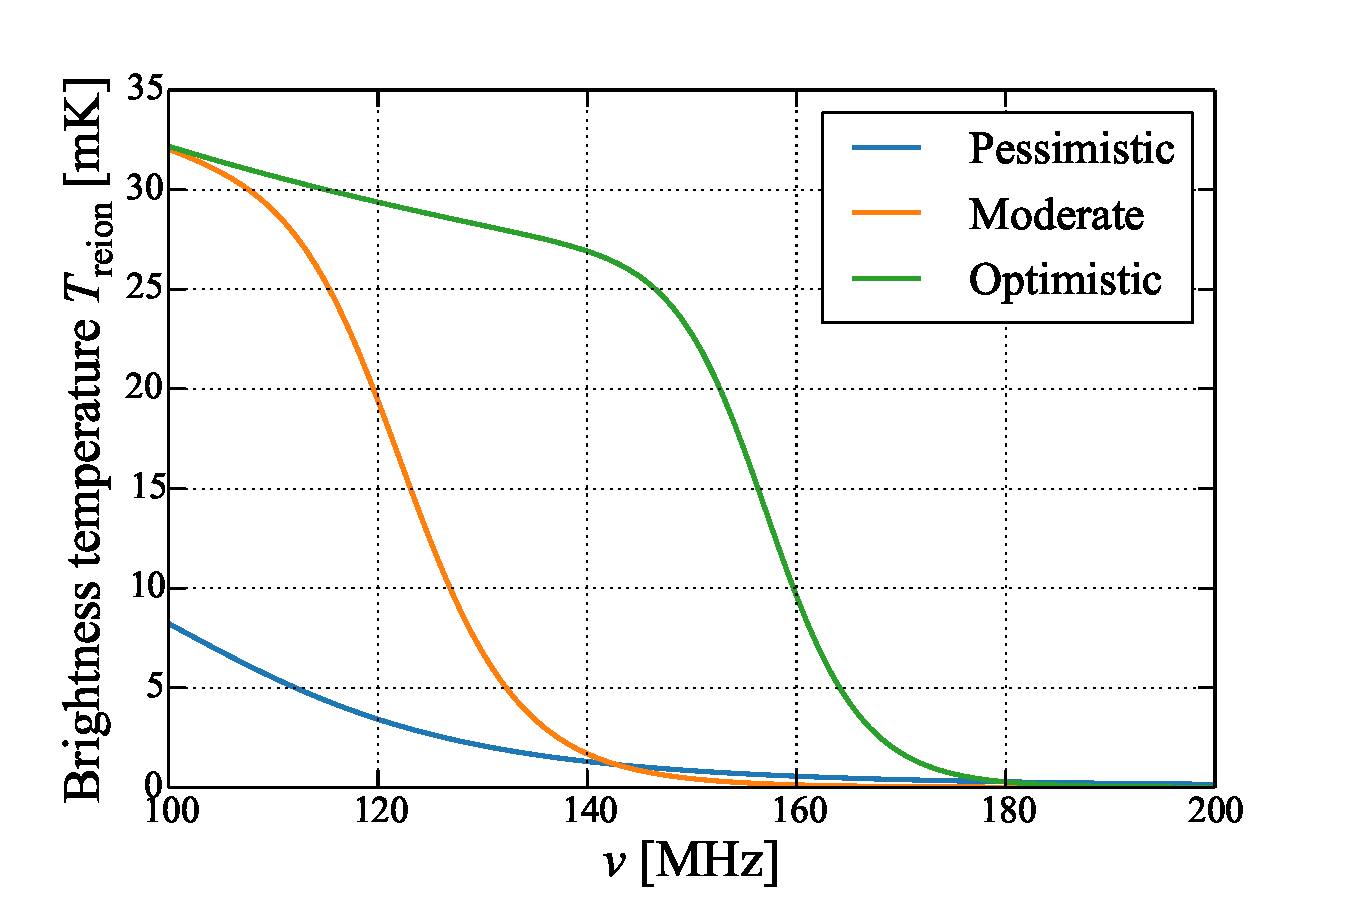
\includegraphics[width=0.5\textwidth]{figures/reionScenarios.pdf}
	\caption{\acl{Fill this in.}}
	\label{fig:reionScenarios}
\end{figure}


\begin{figure}[h]
	\centering
	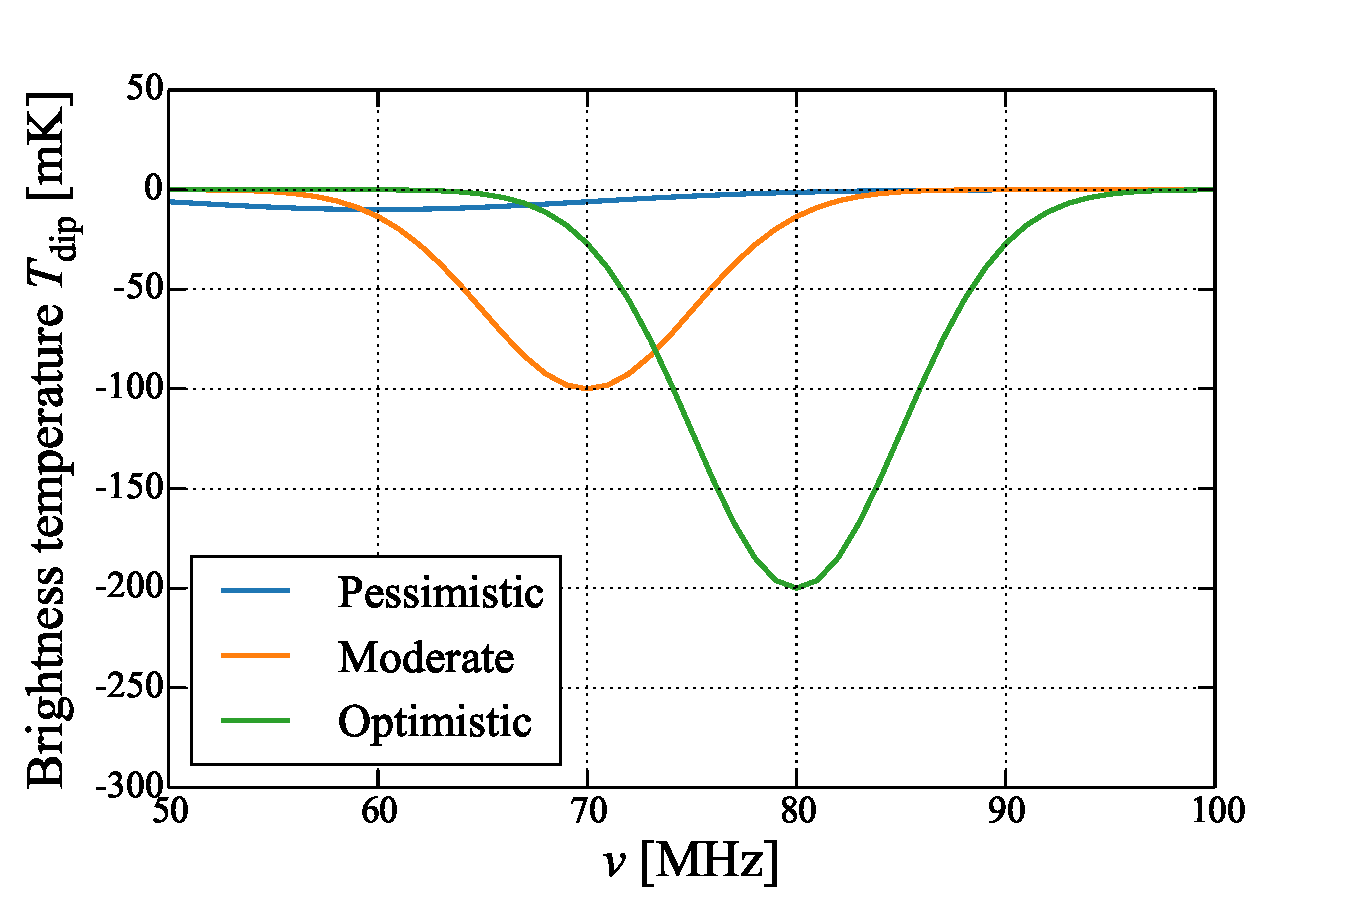
\includegraphics[width=0.5\textwidth]{figures/dipScenarios.pdf}
	\caption{\acl{Fill this in.}}
	\label{fig:dipScenarios}
\end{figure}

The errors on final model parameters will depend on the fiducial ``true" values that are used in our simulations. We consider three different reionization scenarios:
\begin{itemize}
\item Pessimistic reionization scenario, with $(T_{21}, z_r, \Delta z) = (10\,\textrm{mK}, 12, 3) $. With reionization occurring in a rather extended fashion at relatively high redshifts, this scenario should be the most difficult one to detect, since foregrounds are brighter at high redshifts. Additionally, an extended reionization scenario more closely mimics smooth foregrounds.
\item Moderate reionization scenario, with $(T_{21}, z_r, \Delta z) = (27\,\textrm{mK}, 10.5, 0.8) $. This model is motivated by the best-fit value of $z_r$ from \acl{Cite WMAP}. The value of $T_{21}$ is taken from theoretical calculations \acl{Cite Jonathan}, while $\Delta z$ is chosen to be neither too extended nor too abrupt.
\item Optimistic reionization scenario, with $(T_{21}, z_r, \Delta z) = (27\,\textrm{mK}, 8, 0.5) $. Here we choose to roughly match expectations from recent results from optical and infrared observations, which (in contrast to results from CMB experiments) typically favor reasonably rapid reionization at lower redshifts.
\end{itemize}
Similarly, we consider three different pre-reionization scenarios of varying degrees of optimism, although without the CMB as a guide in the pre-reionization era, the parameters are somewhat more arbitrary:
\begin{itemize}
\item Pessimistic pre-reionization scenario, with $(A, \nu_0, \Delta z) = (10\,\textrm{mK}, 60\,\textrm{MHz}, 10\,\textrm{MHz}) $.
\item Moderate pre-reionization scenario, with $(A, \nu_0 \Delta z) = (100\,\textrm{mK}, 70\,\textrm{MHz}, 5\,\textrm{MHz}) $.
\item Optimistic pre-reionization scenario, with $(A, \nu_0, \Delta z) = (200\,\textrm{mK}, 80\,\textrm{MHz}, 5\,\textrm{MHz}) $.
\end{itemize}

%\begin{figure*}[h]
%	\centering
%	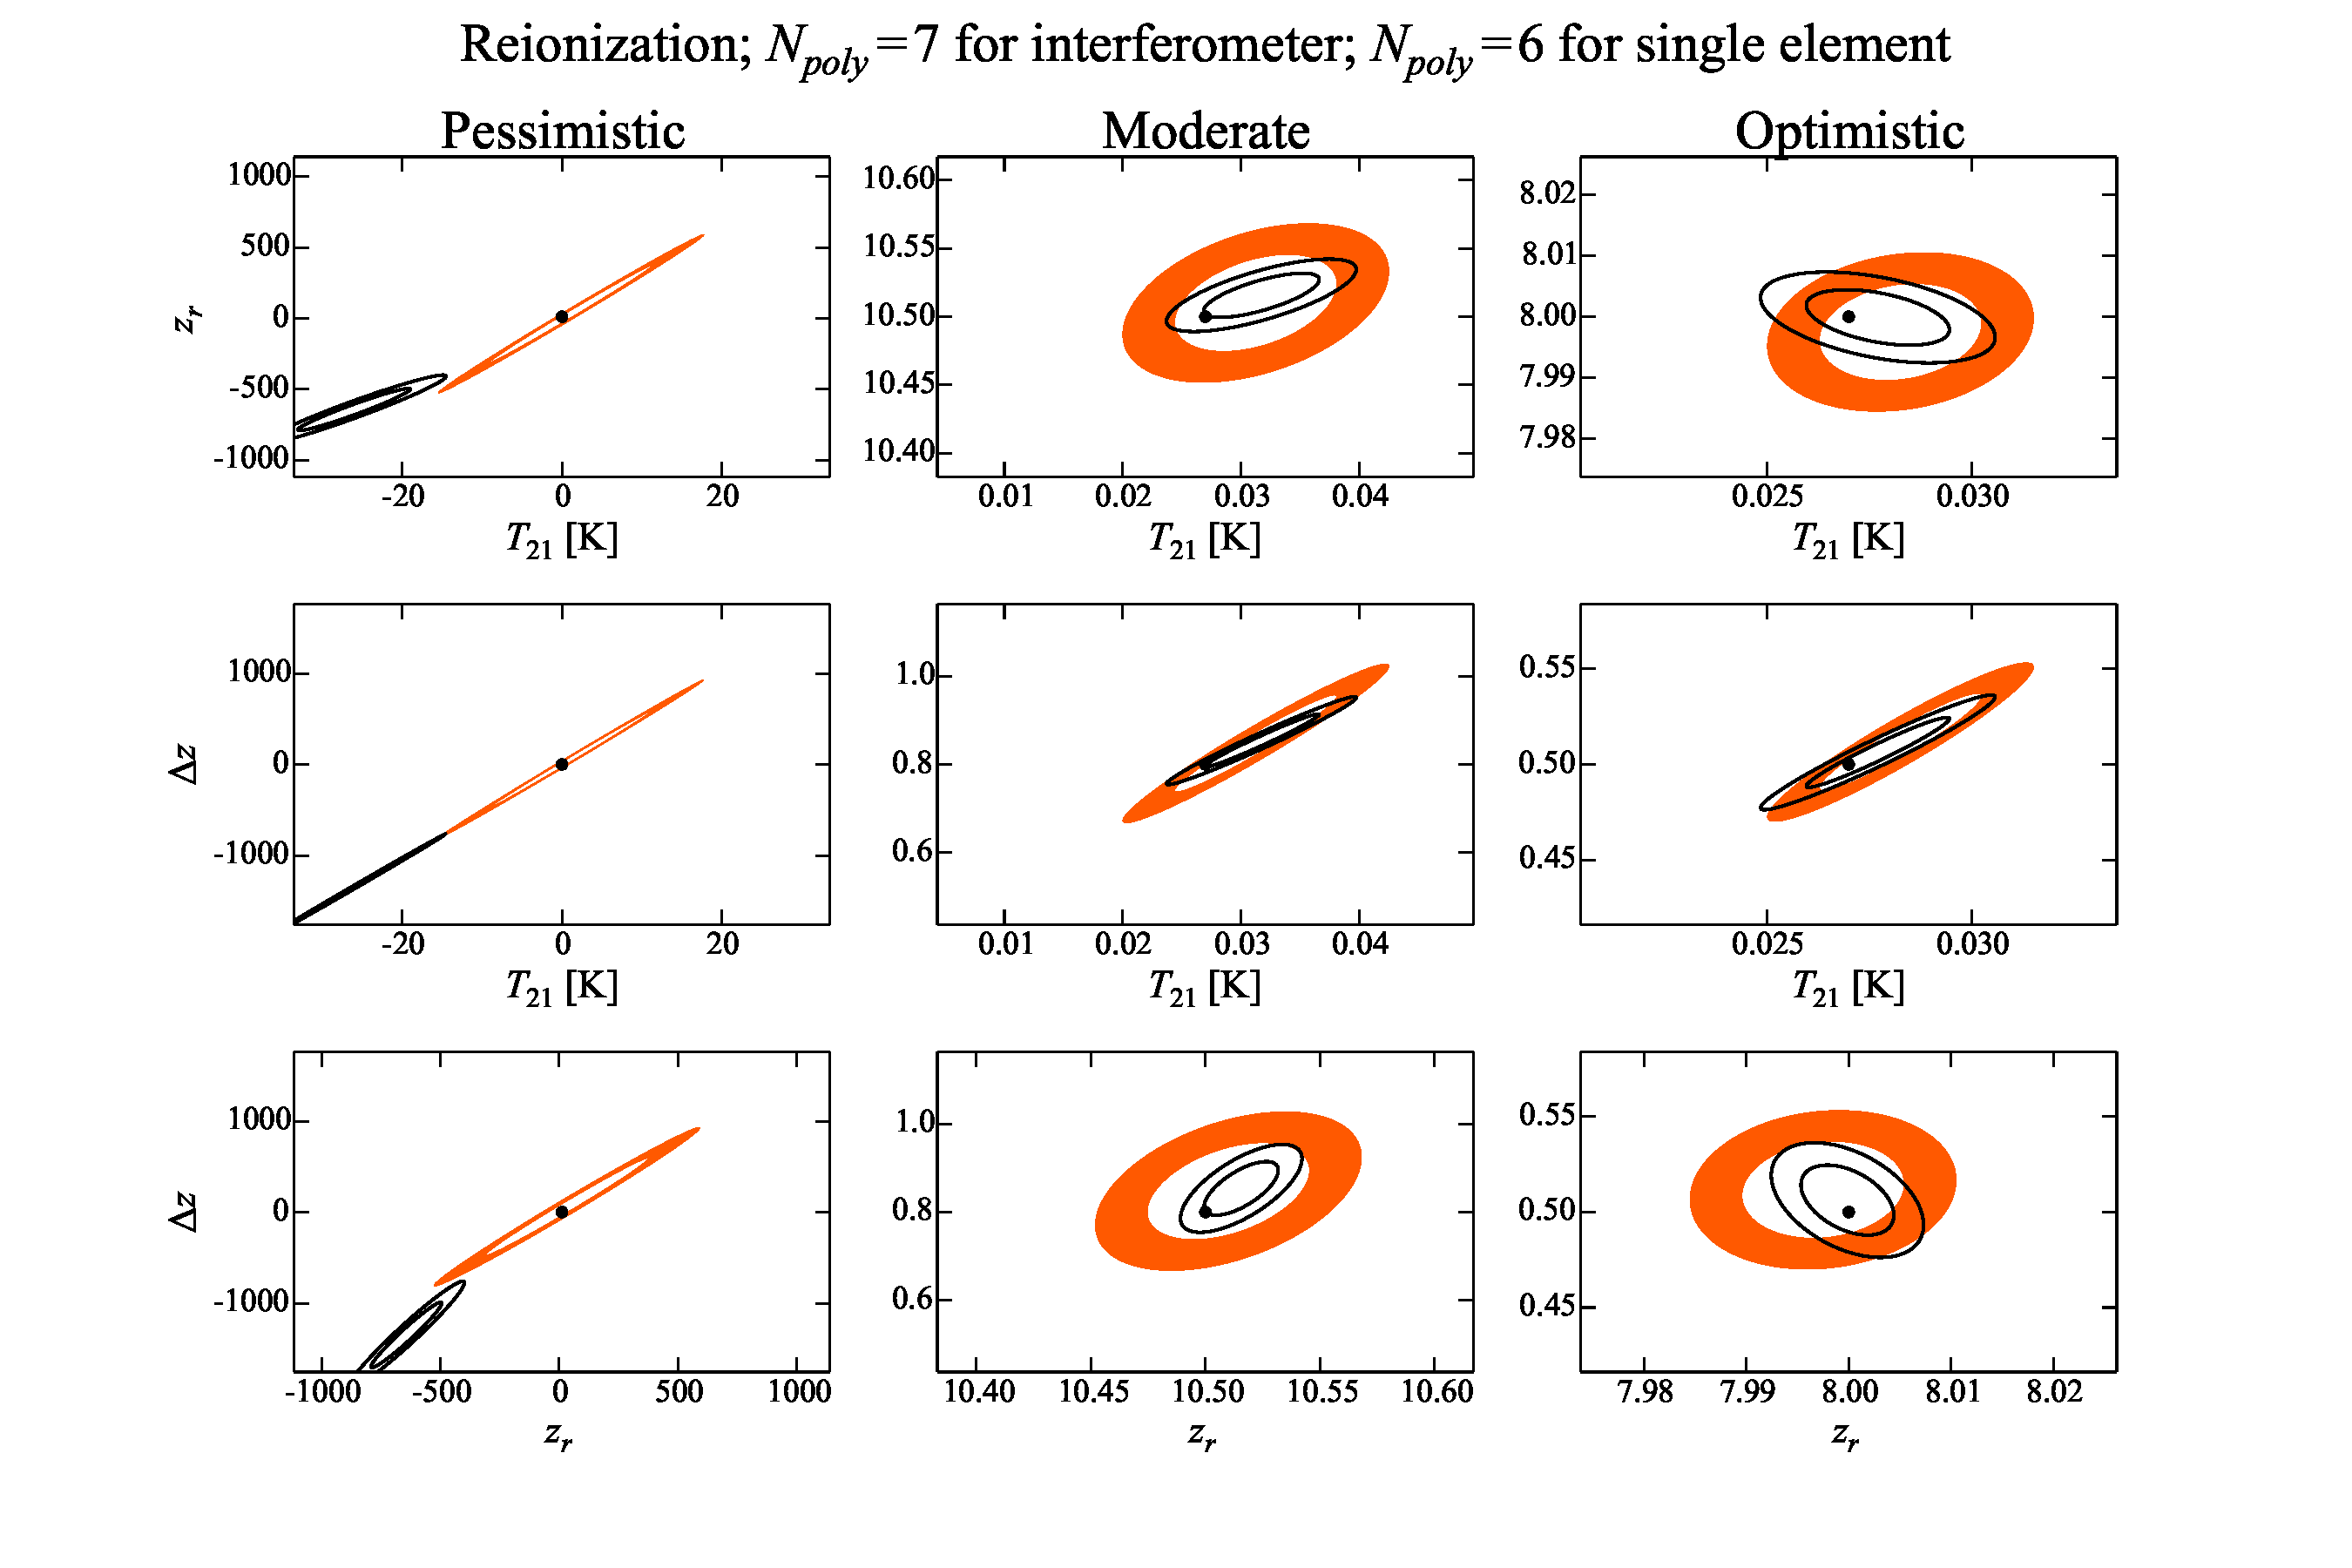
\includegraphics[width=1.00\textwidth,trim=3cm 2cm 3cm 0cm,clip]{figures/reionContoursPoly7Poly6.pdf}
%	\caption{\acl{Fill this in. Polynomial order was 7, and integration time was 300 hours. Also need to rerun for smaller array and smaller beam}}
%	\label{fig:reionContoursPoly7Poly6}
%\end{figure*}
\begin{figure*}[t]
	\centering
	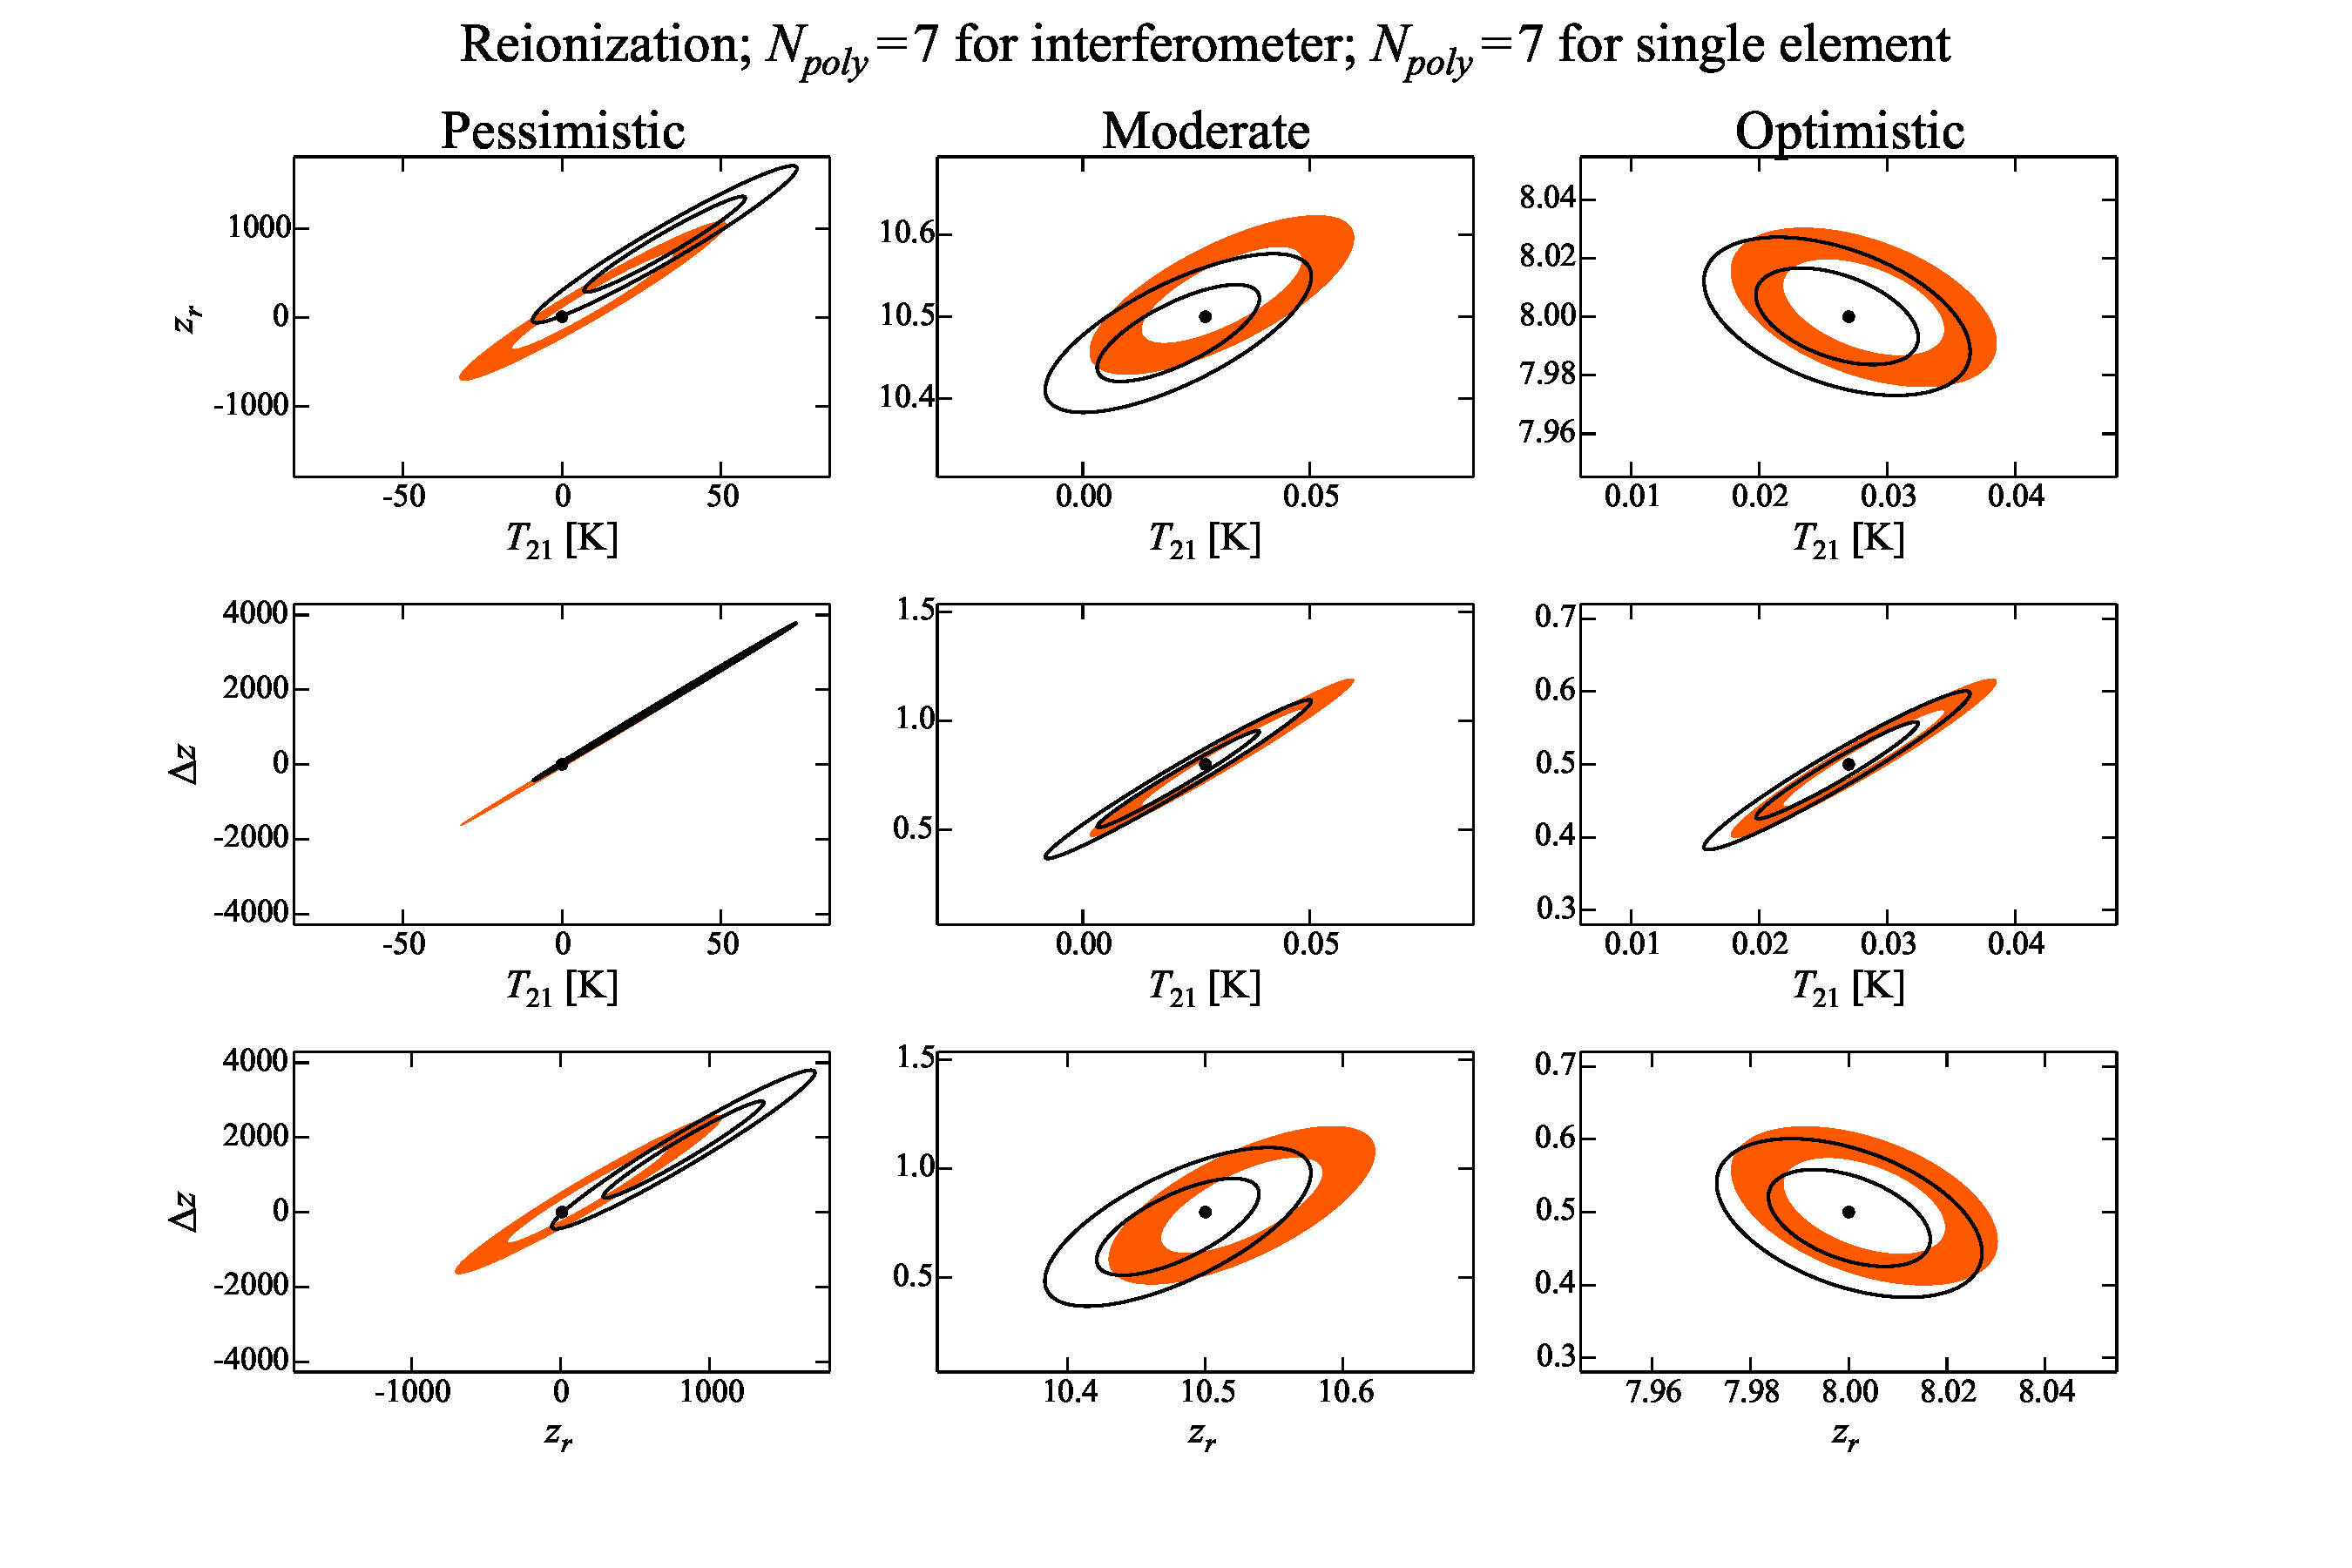
\includegraphics[width=1.00\textwidth,trim=3cm 2cm 3cm 0cm,clip]{figures/reionContoursPoly7Poly7.pdf}
	\caption{\acl{Fill this in. Polynomial order was 7, and integration time was 300 hours. Also need to rerun for smaller array and smaller beam}}
	\label{fig:reionContoursPoly7Poly7}
\end{figure*}


\begin{figure*}[t]
	\centering
	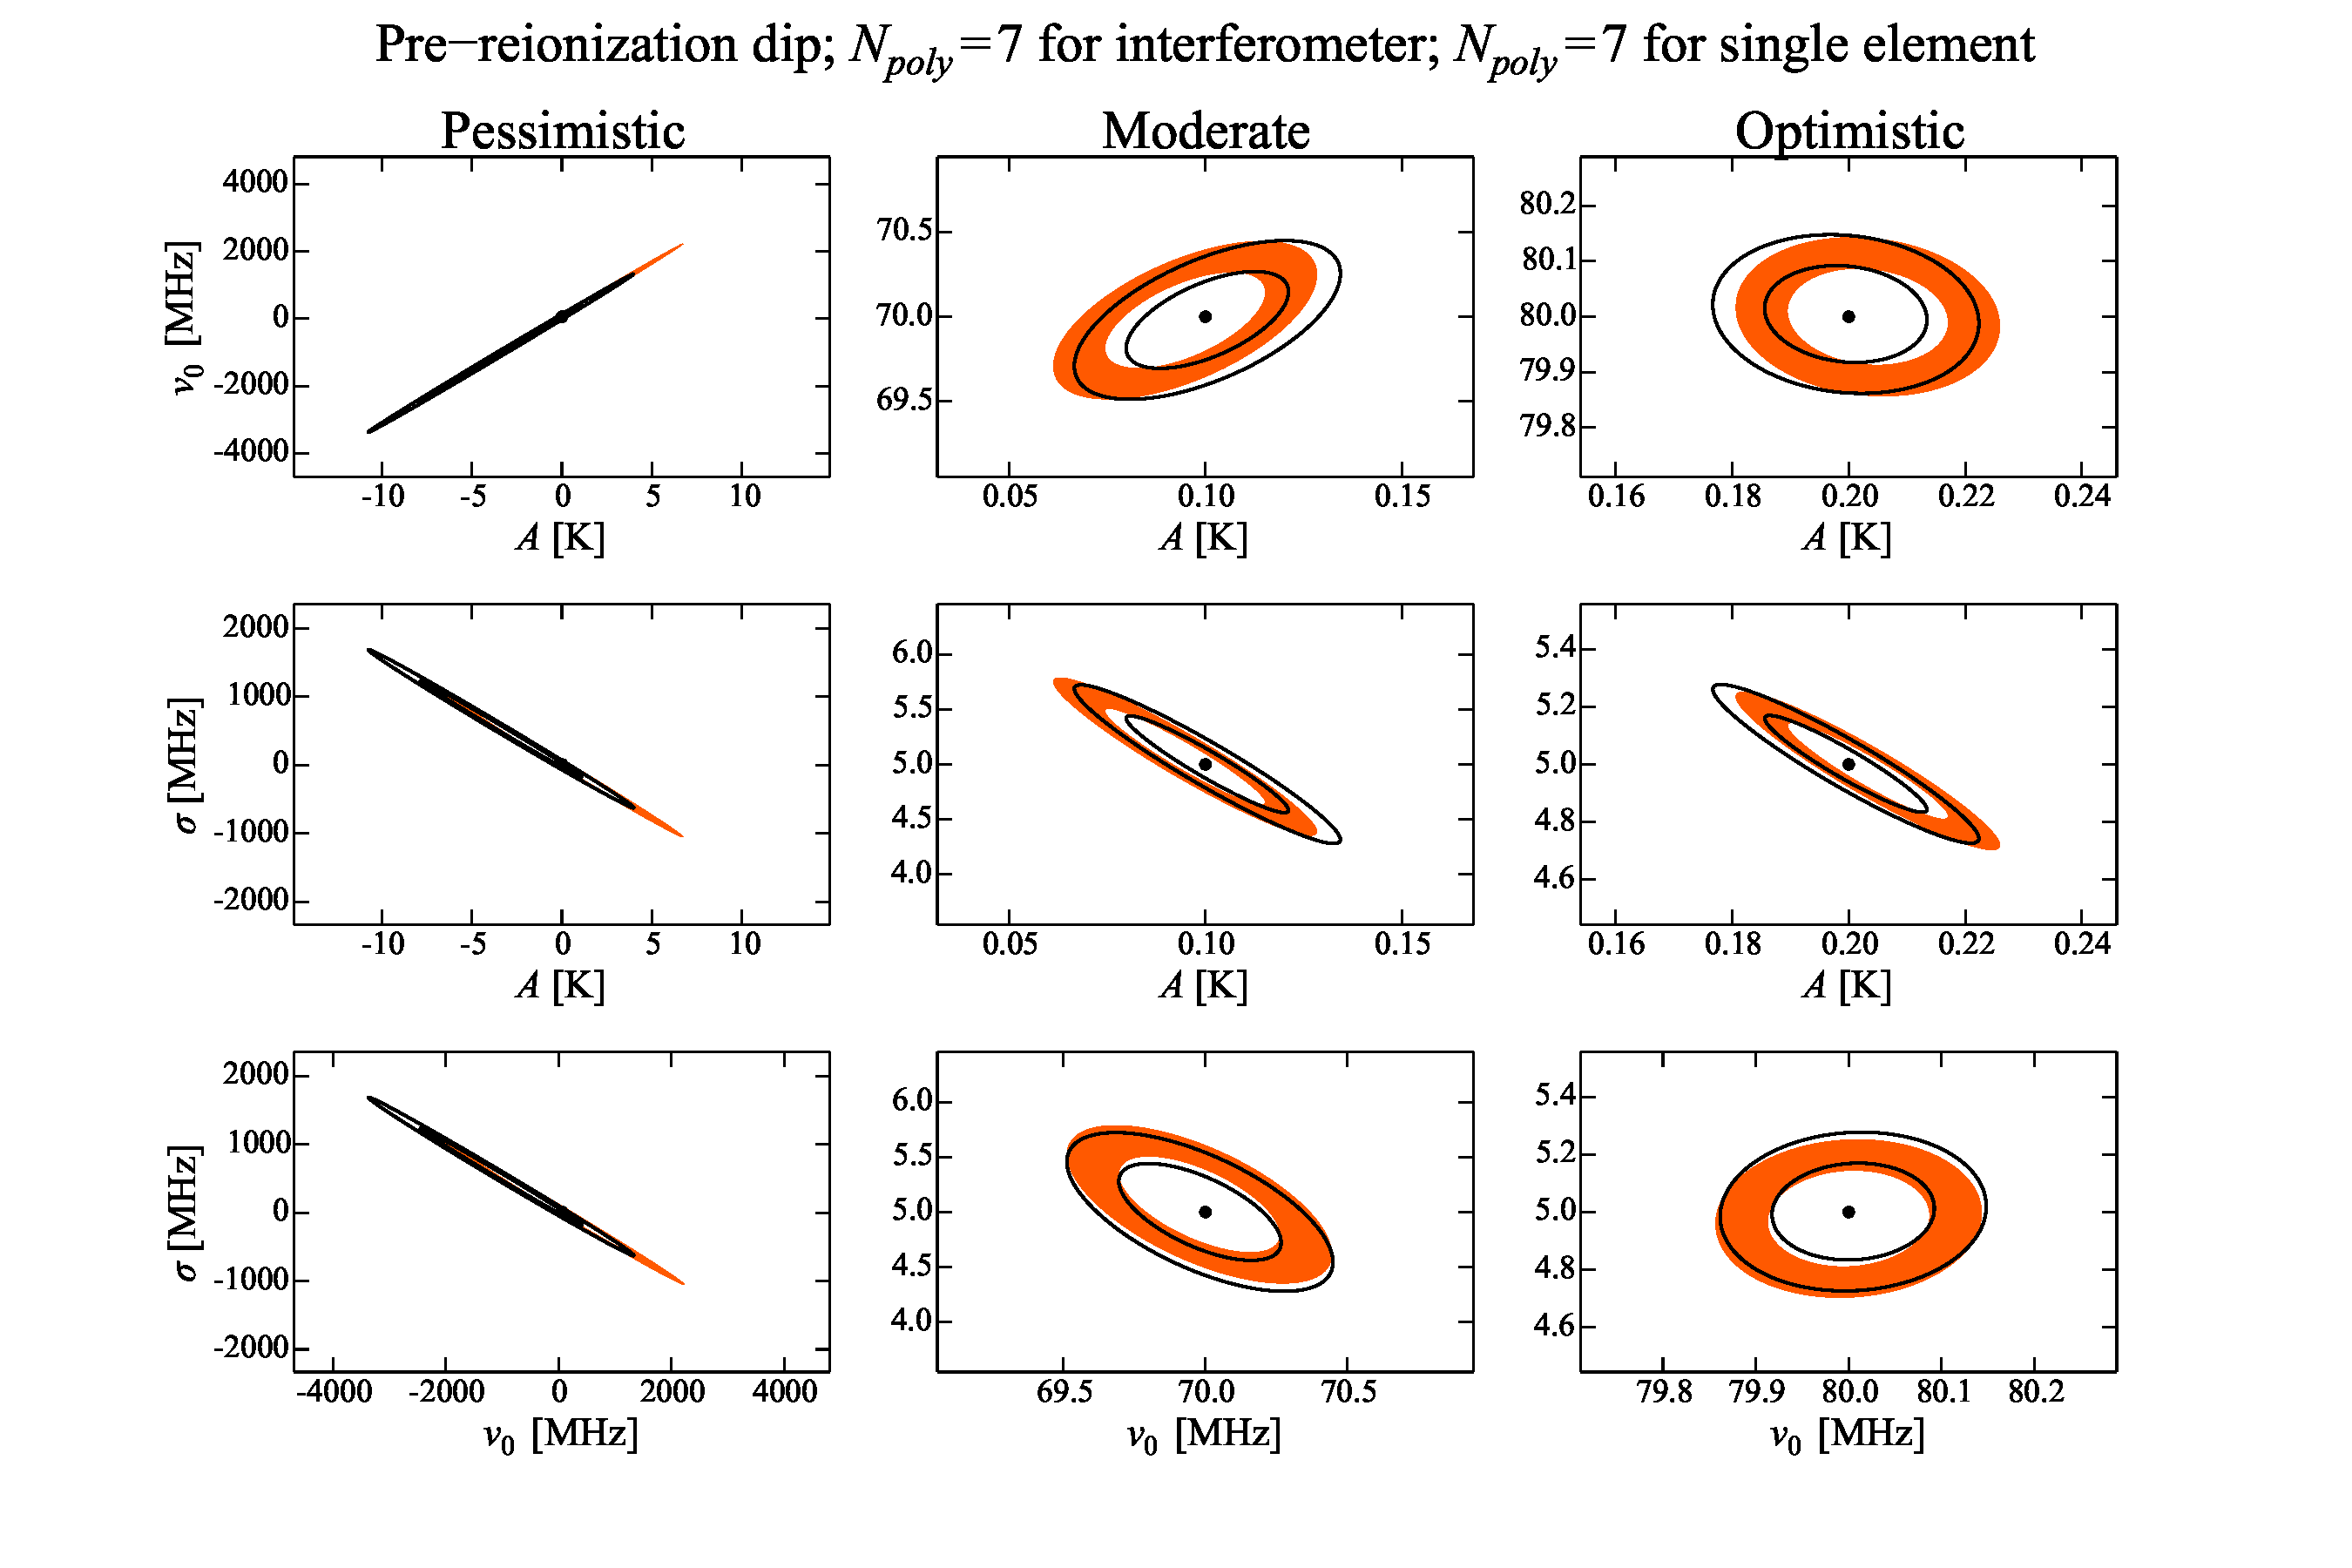
\includegraphics[width=1.00\textwidth,trim=3cm 2cm 3cm 0cm,clip]{figures/dipContoursPoly7Poly7.pdf}
	\caption{\acl{Fill this in. Polynomial order was 7, and integration time was 300 hours. Also need to rerun for smaller array and smaller beam}}
	\label{fig:dipContoursPoly7Poly7}
\end{figure*}

These scenarios are depicted in Figurse \ref{fig:reionScenarios} and  \ref{fig:dipScenarios}. The corresponding model parameters are summarized in Table \acl{Do this}, along with the associated Fisher matrix projections for each parameter's $1\sigma$ error bars after having marginalized over the other parameters. Pairwise parameter contours are shown in Figures \ref{fig:reionContoursPoly7Poly7} and Figures \ref{fig:dipContoursPoly7Poly7}. The results for single dipole experiments are shown using the filled regions, with orange portions signifying $95\%$ confidence regions and the enclosed white portions signifying $68\%$ confidence regions. Solid lines demarcate the corresponding confidence regions for our interferometer. For both types of experiment, we found that setting the polynomial order $N_\textrm{poly}$ to $7$ gave biases subdominant to the errors. The black point in each plot shows the fiducial (``true") parameter values used.

Immediately obvious is the fact that the pessimistic scenarios will be extremely difficult to measure, whether using an interferometer or a single element. 
With those scenarios, the cosmological signals are simply too extended, and occur at too high redshifts for them to be easily distinguished from the bright foregrounds. Encouragingly, we see that both the moderate and the optimistic scenarios should be detectable by both types of instrument. Importantly, one sees that the interferometer performs just as well as the single-element experiment does, suggesting that an interferometric measurement of the global signal may be a interesting viable alternative.


% Requires the booktabs if the memoir class is not being used
\begin{table*}[htbp]
   \centering
   %\topcaption{Table captions are better up top} % requires the topcapt package
   \begin{tabular}{@{} llcccccc @{}} % Column formatting, @{} suppresses leading/trailing space
      \toprule
      & & \multicolumn{3}{c}{Reionization} & \multicolumn{3}{c}{Pre-reionization Dip} \\
      \cmidrule(lr){3-5} % Partial rule. (r) trims the line a little bit on the right; (l) & (lr) also possible
      \cmidrule(lr){6-8} 
      Model &  & $T_{21}$ [mK] & $z_r$ & $\delta z$ & $A$ [mK] & $\nu_0$ [MHz] & $\sigma$ [MHz]\\
      \midrule
      Pessimistic & Fiducial Value & 10 & 12 & 3 & 10 & 60 & 10 \\
      			 & Interferometer Error & $\pm16$ & $\pm356$ & $\pm855$ & $\pm2$ & $\pm949$ & $\pm468$ \\
      			 & Single Dipole Error  & $\pm16$ & $\pm360$ & $\pm854$ & $\pm2$ & $\pm930$ & $\pm461$ \\
%      \midrule
%      Moderate & Interferometer & 0.01180649 & 0.03890324 & 0.146714 & 0.01365896 & 0.18902933 & 0.2904813 \\ 
%                     & Single Dipole & 0.01171378 & 0.03891129 & 0.14587114 & 0.0135119 & 0.18800803 & 0.28876988 \\
%      \midrule 
%      Optimistic & Interferometer & 0.00418164 & 0.01088959 & 0.04390254 & 0.00920051 & 0.05771563 & 0.11111618 \\ 
%                     & Single Dipole & 0.00416954 & 0.01092319 & 0.04383557 & 0.00911918 & 0.05767337 & 0.11057458 \\
      \bottomrule
   \end{tabular}
   \caption{Table of parameters and error bars for different reionization scenarios and experiments.}
   \label{tab:booktabs}
\end{table*}

%
%\section{Monte carlo / foreground simulation results}
%\label{sec:MonteCarlos}
%
%
%\begin{itemize}
%\item $\mathbf{N}_\textrm{fg}$ might not be properly modeled, so we can't use $[\mathbf{Q}^\dagger \mathbf{N}^{-1} \mathbf{Q}]^{-1}$ as a reliable indicator of the errors.  (Although recall that it's a perfectly fine choice for extracting the signal).
%\item To get reliable estimates...Monte Carlo!
%\item Really great results! (Error bars and covariance on the recovered spectra).
%\end{itemize}
%
%Recall from Section \ref{sec:MathForm} that using the least-squares method for recovering $\xhat$ allows us to analytically determine the error covariance of $\xhat$ via Equation \eqref{eqn:Covxhat}. However, this formula for the covariance is only true if we exactly know the noise covariance matrix. Thus, since $\Nfg$ might not be properly modeled, we must still resort to Monte Carlo simulations to determine the error bars on our measurements. 
%
%Our Monte Carlo simulations generate many visibilities $V(\mathbf{b}_i)$ from randomly perturbed sky models. \mep{Is ``randomly perturbed'' an appropriate way to describe it?} The sky models are derived by taking the all-sky survey from \citet{Haslam_408MHz_map} and using the power-law model of the foreground spectrum used in \citet{Liu_21cm_Fg} to extrapolate a map at the desired frequency. For a pixel at $\boldsymbol \theta$, the brightness at a certain frequency $\nu$ is 
%\begin{equation}
%I(\boldsymbol \theta) = I_H(\boldsymbol \theta) \left ( \frac{\nu}{\nu_H} \right ) ^{-\alpha + \Delta \alpha}
%\end{equation}
%where $I_H$ is the sky map from \citet{Haslam_408MHz_map}, $\nu_H=408$MHz, $\alpha = 2.8$, and $\Delta \alpha$ is a perturbing index randomly generated with variance 0.1. From this model, we can generate a vector of visibilities for all of the different baselines in an array. This vector is $\y$ from Equation \eqref{eqn:yQxn}. The visibilities are defined as 
%\begin{equation}
%V(\mathbf{b}_i) = \int d \Omega A(\boldsymbol \theta) I(\boldsymbol \theta) e^{-2\pi i\frac{\nu}{c} \mathbf{b}_i \cdot \boldsymbol \theta}
%\end{equation}
%where $\boldsymbol \theta$ is the angular position on the sky, $A$ is the primary beam for the antennas, $\mathbf{b_{\textit{j}}}$ is the $j$th baseline, $\nu$ is the frequency of observation, and $I$ is the intensity \mep{What's the correct name for this?} of the sky model. 
%
%Once we have generated a $\y$ vector, we can use Equation \eqref{eqn:xhat} to find the estimator for the global signal that our analysis would produce for that particular sky. The variance of a large set of estimators from many such sky models provides us with the error bars for an experiment measuring the global signal. \mep{I don't like the phrasing of this paragraph.} 

%\section{Fisher matrix results}
%\label{sec:Fisher}
%\begin{itemize}
%\item Fisher matrix formalism for translating error statistics from recovered spectra to parameterizations of the signal.
%\end{itemize}
%
%
%\mep{Insert figures of pairwise projections and discussion thereof.} 
%
%\begin{figure}[h]
%	\centering
%	%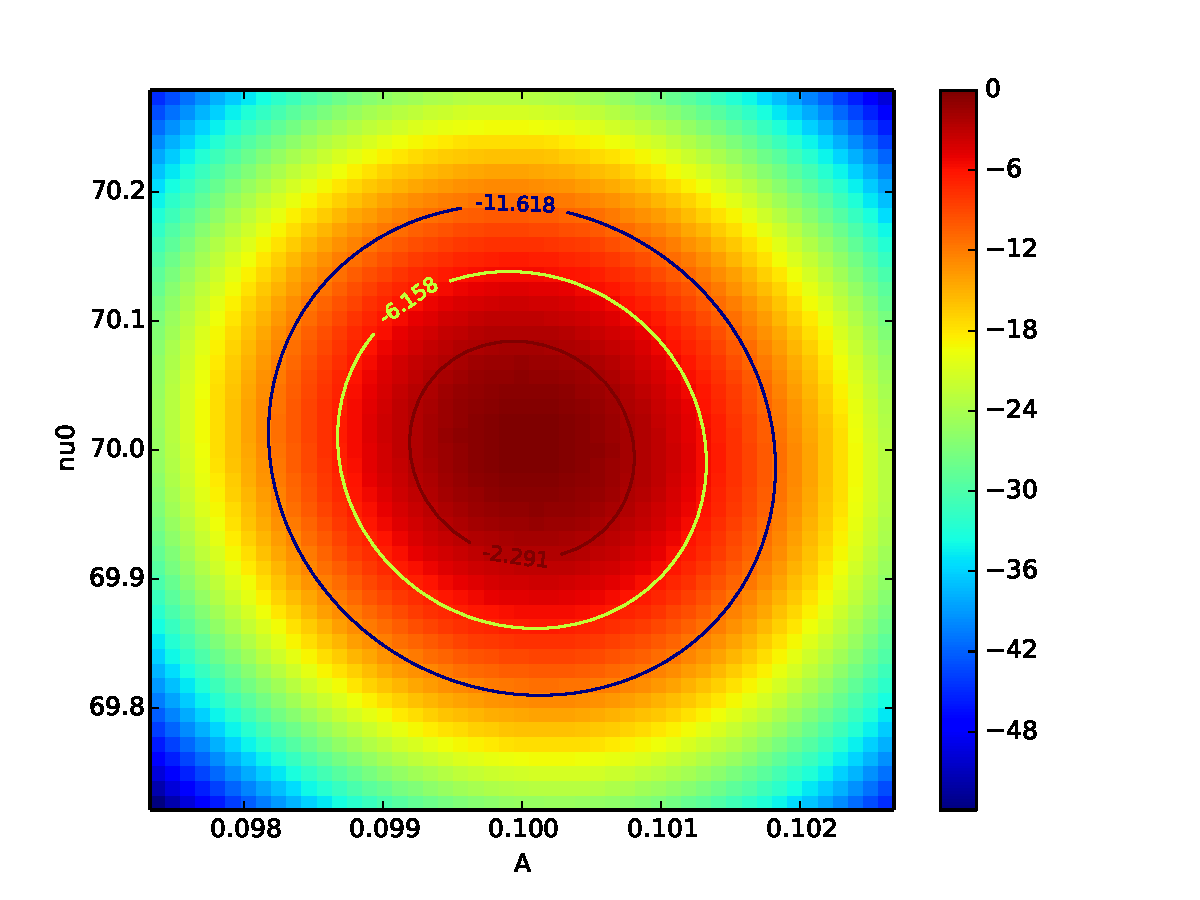
\includegraphics[width=0.55\textwidth]{figures/oldFigures/contours_A_nu0.pdf}
%	\caption{\acl{Fill this in.  Probably also want to make this a horizontal stripe of constraints.}}
%	\label{fig:contours}
%\end{figure}
%
%\begin{figure}[h]
%	\centering
%	%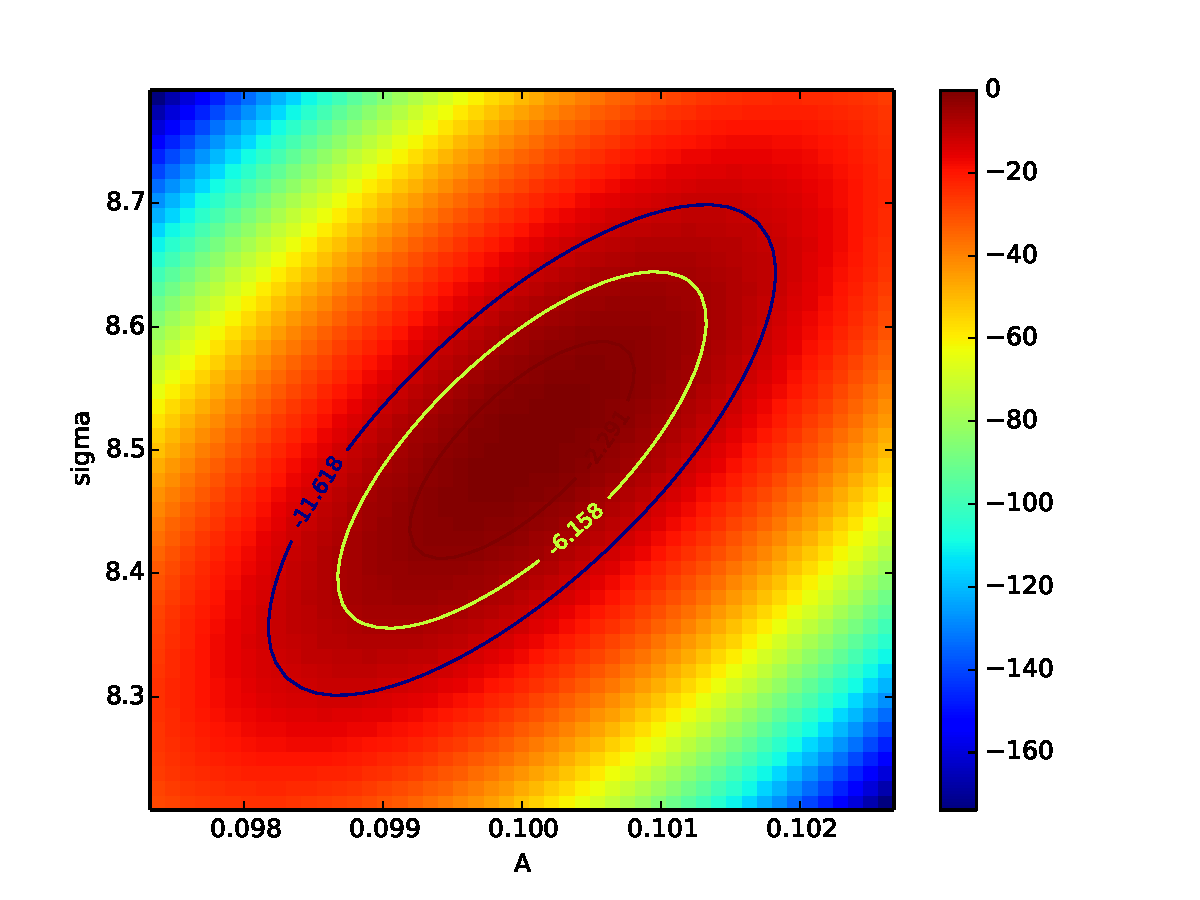
\includegraphics[width=0.55\textwidth]{figures/oldFigures/contours_A_sigma.pdf}
%	\caption{\acl{Fill this in}}
%\end{figure}
%
%\begin{figure}[h]
%	\centering
%	%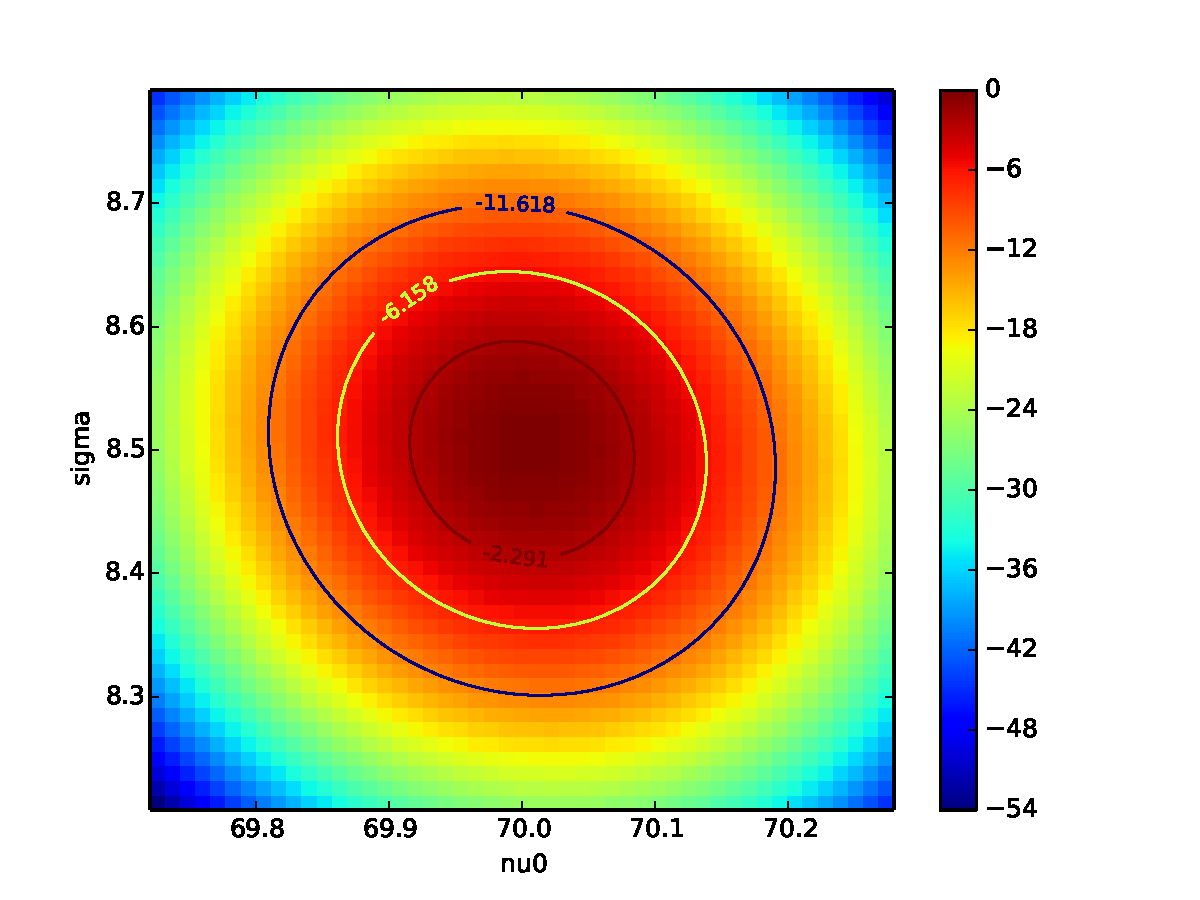
\includegraphics[width=0.55\textwidth]{figures/oldFigures/contours_nu0_sigma.pdf}
%	\caption{\acl{Fill this in}}
%\end{figure}

\section{Conclusions}
\label{sec:Conc}
\acl{On the theme of better relating this to a broad audience, we can also relate this to the high redshift galaxy people.  If their (collective) constraints are to be believed, there should be a sharp rise in ionization fraction at a redshift that's *just* below what EDGES is able to constrain.  So perhaps this can be motivation for building a global signal experiment that can confirm/refute the optical and IR people}
\begin{itemize}
\item This is a great way to do this measurement.  It will produce lots of great science! And eternal glory!
\end{itemize}

%\bf Reverse Outline \rm \mep{mostly for my use in writing the conclusion}
%\begin{itemize}
%\item The purpose of our paper is to explore ``a general theory of interferometric measurements of the global 21 cm signal.'' 
%\item General Principles of Array Design
%	\begin{itemize}
%	\item ``The optimal baseline consists of antennas that are placed as close together as is physically possible.''
%	\item We found the optimal beam size for each element of the array to be $\sim25^\circ$ (FWHM).
%	\item The array does not have to be large; even a small $3\times3$ or $4\times4$ grid array would be as sensitive as a single dipole experiment.
%	\end{itemize}
%\item Data Analysis 
%	\begin{itemize}
%	\item General Method: 1) Estimate the spatial monopole at each frequency channel. 2) Combine into a global signal spectra and again subtract the foreground. 
%	\item If during step 1 we choose a data analysis method that minimizes $\chi^2$ (as was used by LOFAR \mep{Keep this only if we add that discussion at the end of Sec. \ref{sec:badMmatrix}}) while simultaneously following the design principles in Sec. \ref{sec:BackOfEnvelopeArrayDesign}, we must use a pseudo-inverse that tends to imprint sharp spectral features into the estimate of the global signal. 
%	\item Therefore, we propose an alternative method that minimizes the variance \mep{Do I need to add that caveat about $\N$ here?} and preserves the amplitude of a pure monopole sky. 
%	\item This method will leak information from higher modes into the estimator of the global signal; however this turns out to be advantageous, as the leaked information aides in subtracting the monopole component of the foregrounds.
%	\item Also, if the array is built to the specifications detailed in Sec. \ref{sec:BackOfEnvelopeArrayDesign}, then the array will not be sensitive to cosmological anisotropies. Thus, the leakage will not add contaminants of cosmological origin. 
%	\item We recommend choosing our noise-covariance matrix $\N$ to be the identity, as a foreground-motivated $\N$ does not significantly remove foreground bias in observations away from the galactic plane and can also imprint harmful spectral artifacts into the data. 
%	\item Moving on to step 2, we choose to fit foreground and cosmological model parameters simultaneously in order to provide a description of signal loss in foreground subtraction. 
%	\end{itemize}
%\item Simulation Results!
%
%\end{itemize}

In this paper, we explored a general methodology for using an interferometer to measure the global 21 cm signal. First we used a toy model of an array to develop general design principles for a global 21 cm experiment. We found that an optimal array design consists of a small grid of closely packed antennas, each with a FWHM beam size of $\sim25^\circ$. 

Next we examined the choices we could make in data analysis. We chose a two-step process for our general analysis method: first we estimated the spatial monopole at each frequency channel; then we combined the estimates into a single global signal spectra and performed a final foreground subtraction. During the first step, we found that if we chose a data analysis method that minimized $\chi^2$ while simultaneously following the design principles in Section \ref{sec:BackOfEnvelopeArrayDesign}, we would be forced to use a pseudo-inverse that would imprint sharp spectral features into the estimate of the global signal. Therefore, we propose an alternative method that instead minimizes the variance \mep{Do I need to add that caveat about $\N$ here?} and also preserves the amplitude of a pure monopole sky. This method will leak information from higher modes into the estimator of the global signal; however this turns out to be advantageous, as the leaked information aides in subtracting the monopole component of the foregrounds. Also, if the array is built to the specifications detailed in Section \ref{sec:BackOfEnvelopeArrayDesign}, then the array will not be sensitive to contaminates from cosmological anisotropies. We recommend against choosing a foreground-motivated noise covariance, as it does not significantly remove foreground bias in observations away from the galactic plane and can also imprint harmful spectral artifacts into the data. In the second step, we choose to fit foreground and cosmological model parameters simultaneously in order to provide a description of signal loss in foreground subtraction. 

Putting our array design and data analysis method into numerical simulation, we find that a measurement by an interferometer is comparable to a single dipole experiment. Both methods require 7th order polynomials for foreground models and will be able to constrain [parameters] to within [values]. \mep{add more quantitative stuff once new figs arrive} Therefore, an interferometric measurement of the global 21 cm signal is worth exploring as an alternative to a single dipole experiment for finding stringent constraints on the dark ages and epoch of reionization. 

\section{Acknowledgements}
\acl{Acknowledge Carina and NERSC}
\mep{Looking at your other papers for what should go here. Seems like you need a contract \# for nersc. Any funding sources that should be added?}
It brings the authors great pleasure to thank Carina Cheng and Zaki Ali for useful discussions. This research used resources of the National Energy Research Scientific Computing Center, which is supported by the Office of Science of the U.S. Department of Energy under Contract No. BLANK. 


\appendix
\section{Proof of minimum-variance property of global signal estimator}
\label{minVarProof}
\acl{Check generality wrt H}
In this Appendix, we provide a constructive proof that choosing $\M$ to be diagonal (as we do in this paper starting in Section \ref{sec:BetterM}) minimizes the variance of our estimator $\xhat$, provided $\N$ represents the covariance of our measurement, i.e., $\N = \langle \mathbf{y} \mathbf{y}^\dagger \rangle - \langle \mathbf{y} \rangle \langle \mathbf{y} \rangle^\dagger$. \acl{I'm trying to figure out how to make this more self-contained and say what xhat is here.} As discussed in Section \ref{sec:SimResults}, the general form for the covariance $\boldsymbol \Sigma$ of $\xhat$ follows from Equation \eqref{eqn:xhat}, and is given by
\begin{equation}
\boldsymbol \Sigma \equiv \langle \xhat \xhat^\dagger \rangle - \langle \xhat \rangle \langle \xhat \rangle^\dagger = \M \Q^\dagger \N^{-1} \Q \M \equiv \M \mathbf{B} \M^\dagger,
\end{equation}
where we have made the definition $\mathbf{B} \equiv \Q^\dagger \N^{-1} \Q$ for convenience. With this notation, the window function matrix becomes $\W = \M \mathbf{B}$.

To derive a minimum-variance estimator, we minimize the diagonal elements of $\boldsymbol \Sigma$ subject to the constraint that the window functions satisfy $\W_{ii} = (\M \mathbf{B})_{ii} =1$. Introducing a Lagrange multiplier $\lambda_i$, we seek to minimize the quantity
\begin{equation}
L = (\M \mathbf{B} \M^\dagger)_{ii} - \lambda_i  (\M \mathbf{B})_{ii}.
\end{equation}
Differentiating with respect to the real and imaginary parts of a generic component $\M_{jk}$ of $\M$, one obtains
\begin{equation}
\frac{\partial L}{\partial \textrm{Re} \M_{jk}} = (\mathbf{B} \M^\dagger + \M \mathbf{B})_{jk} - \lambda_j \mathbf{B}_{kj} =0
\end{equation}
and
\begin{equation}
\frac{\partial L}{\partial \textrm{Im} \M_{jk}} = (\mathbf{B} \M^\dagger - \M \mathbf{B})_{jk} - \lambda_j \mathbf{B}_{kj} =0,
\end{equation}
where we have set each expression to zero in order to perform a minimization. Now, recall that $\mathbf{B}$ is Hermitian. However, the combination $\mathbf{B} \M^\dagger - \M \mathbf{B}$ is by construction anti-Hermitian. For the second equation to hold, then, we require that $\mathbf{B} \M^\dagger = \M \mathbf{B}$, so that the anti-Hermitian portion vanishes identically. With this, the first equation reduces to $2 \M \mathbf{B} = \boldsymbol \Lambda \mathbf{B}$, where $\boldsymbol \Lambda_{ij} = \lambda_i \delta_{ij}$. Acting on both sides with $\mathbf{B}^{-1}$ then gives $\M = \boldsymbol \Lambda / 2$, which tells us that $\M$ must be diagonal. To fix the values of the Lagrange multipliers along the diagonal, we use our constraint $\W_{ii} = (\M \mathbf{B})_{ii} =1$ to obtain $\M_{ij} = \delta_{ij} / \mathbf{B}_{ii}$. Recalling the definition of $\mathbf{B}$, we see that this is precisely the form of Equation \eqref{eq:diagM}, completing our proof.

\section{Global signal Fisher matrix forecasting methods}
\label{fisher}
In this Appendix, we review the Fisher matrix formalism used in \acl{Cite Gianni} to forecast the error bars and biases in a global signal measurement. We do not claim any originality here, and include a description of the formalism only for completeness.

Suppose we group our final estimate of the global signal $\widehat{T}_0 (\nu)$ into a vector $\widehat{\mathbf{T}}$, so that each component corresponds to the measured global signal value at a particular frequency. With this notation, the Fisher information matrix is defined as
\begin{equation}
\F_{ij} \equiv -\left \langle \frac{\partial^2 \ln \mathscr{L}(\boldsymbol \theta | \widehat{\mathbf{T}})}{\partial \theta_i \partial \theta_j} \Big{|}_{\boldsymbol \theta_0} \right \rangle
\end{equation}
where $\mathscr{L}(\boldsymbol \theta | \widehat{\mathbf{T}})$ is the likelihood function of a set of model parameters $\boldsymbol \theta$ given the measurements $\widehat{\mathbf{T}}$, with $\boldsymbol \theta_0$ denoting a set of fiducial values for the parameters. Now, recall that $\widehat{\mathbf{T}}$ contains the measured global signal spectrum prior to the smooth foreground fitting described in Section \ref{sec:fitting}. It therefore contains not only the cosmological signal (parameterized by one of the forms given in Section \ref{sec:SimResults}), but also foregrounds and noise, and may be written as
\begin{equation}
\widehat{\mathbf{T}}= \widehat{\mathbf{T}} _\textrm{cosmo} + \widehat{\mathbf{T}}_\textrm{fg} + \boldsymbol \sigma = \boldsymbol \mu (\boldsymbol \theta) +\delta \widehat{\mathbf{T}}_\textrm{fg} + \boldsymbol \sigma,
\end{equation}
where $\widehat{\mathbf{T}} _\textrm{cosmo}$ is the cosmological signal, $\widehat{\mathbf{T}}_\textrm{fg}$ the foregrounds, and $\boldsymbol \sigma$ the residual instrumental noise. In the second equality, we separated the foreground contribution into a portion accounted for by the smooth spectrum fits described in Section \ref{sec:fitting} and a residual, $\delta \widehat{\mathbf{T}}_\textrm{fg}$. The former contribution is combined with the cosmological signal to give a model $\boldsymbol \mu (\boldsymbol \theta)$ for our spectrum. Since this model contains our foreground fits, the parameter vector $\boldsymbol \theta$ records not only the astrophysical/cosmological parameters such as those in Equations \eqref{eq:Dip} and \eqref{eq:Step}, but also the foreground parameters in Equation \eqref{eq:FgFit}. Assuming that the instrumental noise is Gaussian and has zero mean and covariance $\boldsymbol \Pi \equiv \langle \boldsymbol \sigma \boldsymbol \sigma^t \rangle$, the Fisher matrix takes the form
\begin{equation}
\F_{ij} = \frac{\partial \boldsymbol \mu ^t}{\partial \theta_i} \boldsymbol \Pi ^{-1} \frac{\partial \boldsymbol \mu}{\partial \theta_j}.
\end{equation}
Once the Fisher matrix has been computed, the smallest possible error $\Delta \theta_i$ (in the information theoretic sense) on the parameter $\theta_i$ is obtained by calculating $\Delta \theta_i = \sqrt{(\F^{-1})_{ii}}$. While an actual experiment may not necessarily deliver error bars that are as tight as this, the predictions of the Fisher matrix formalism are nonetheless a useful guide for experimental design.

So far, we have only concerned ourselves with the variance of the final parameter constraints. However, foreground residuals will cause more than a spread in the parameter fits --- they will also bias the fits in a systematic way. This bias is given by
\begin{equation}
\delta \theta_i = \sum_{j} (\F^{-1})_{ij} \frac{\partial \boldsymbol \mu ^t}{\partial \theta_j} \boldsymbol \Pi ^{-1} \delta \widehat{\mathbf{T}}_\textrm{fg}.
\end{equation}
In Section \ref{sec:SimResults}, $\delta \xhat_\textrm{fg}$ is obtained by running Monte Carlo simulations. We generate realizations of the foreground sky, which are then fed through a simulation of a measurement and data analysis. Averaging over simulations, the resulting spectra are then fit to logarithmic polynomials. The residuals (i.e., $\delta \widehat{\mathbf{T}}_\textrm{fg}$) are given by Equation \eqref{eq:FgFit}.

%Note that the dimensions here work out because $\delta \xhat$ and $\boldsymbol \mu(\boldsymbol \theta)$ have length $N_\textrm{fq}$, and $C^{-1}$ has dimensions $N_\textrm{fq} \times N_\textrm{fq}$.  
%
%Using the Fisher matrix formalism, we analyzed how well different arrays would be able to constrain models for different epochs in the evolution of the global signal. %\mep{It seems at this point that it would be helpful to refer to a picture of the fiducial model of the global signal, such as the one in your designer's guide paper. Actually, should we in an earlier section describe in more detail what we think the signal will look like? If so, where would that be? In the introduction?} \acl{Yep, I think the intro is the right place for it.  Earlier today I sneakily added a second sentence to the second bullet point there.} 
%At about $z\sim 30$ when the first galaxies form, we expect a significant absorption feature as Lyman-alpha photons couple the spin and gas temperatures (see Fig. \ref{fig:21cmSignal}). This dip can be modeled as a Gaussian in frequency
%\begin{equation}
%\boldsymbol \mu = -A\textrm{exp}\left ( -\frac{(\nu - \nu_0)^2}{2\sigma^2} \right ) 
%\end{equation}
%so that the parameter vector is $\boldsymbol \theta = (A,\nu_0,\sigma)$, where $A$ is the amplitude of the signal, $\nu_0$ is the center of the absorption dip, and $\sigma$ is the width. Given a model and a fisher matrix, we can approximate the likelihood function of the parameter values as a multivariate Gaussian with covariance $\F^{-1}$.  
%\begin{equation}
%L(\boldsymbol \theta) \approx \frac{1}{(2\pi)^{n/2}(\textrm{det} \F^{-1})^{1/2}} \textrm{exp} \left ( -\frac{1}{2}(\boldsymbol \theta - \boldsymbol \theta_{\textrm{m}})^t \F (\boldsymbol \theta - \boldsymbol \theta_{\textrm{m}}) \right )
%\end{equation}
%where $n$ is the length of the parameter vector and $\boldsymbol \theta_{\textrm{m}}$ are the parameters with maximum likelihood. In order to more easily visualize the 3-dimensional contours of $L(\boldsymbol \theta)$, we examine the parameters pairwise by integrating over the third parameter in order to produce a new 2-dimensional likelihood function. Fig. \ref{fig:contours} shows contours of such pairwise likelihood functions for ... 

\bibliographystyle{apj}
\bibliography{globalSig}{}



\end{document}
